%*************************************************************************
% A Classic Thesis Style
% An Homage to The Elements of Typographic Style
%
% Copyright (C) 2017 André Miede and Ivo Pletikosić
%
% If you like the style then I would appreciate a postcard. My address
% can be found in the file ClassicThesis.pdf. A collection of the
% postcards I received so far is available online at
% http://postcards.miede.de
%
% License:
% This program is free software; you can redistribute it and/or modify
% it under the terms of the GNU General Public License as published by
% the Free Software Foundation; either version 2 of the License, or
% (at your option) any later version.
%
% This program is distributed in the hope that it will be useful,
% but WITHOUT ANY WARRANTY; without even the implied warranty of
% MERCHANTABILITY or FITNESS FOR A PARTICULAR PURPOSE.  See the
% GNU General Public License for more details.
%
% You should have received a copy of the GNU General Public License
% along with this program; see the file COPYING.  If not, write to
% the Free Software Foundation, Inc., 59 Temple Place - Suite 330,
% Boston, MA 02111-1307, USA.
%
% PLEASE SEE ALSO THE AUTHORS' NOTE REGARDING THIS LICENSE
% IN THE DOCUMENTATION (ClassicThesis.pdf --> Chapter 1 / Chapter01.tex)
%*************************************************************************
\RequirePackage{silence} % :-\
    \WarningFilter{scrreprt}{Usage of package `titlesec'}
    %\WarningFilter{scrreprt}{Activating an ugly workaround}
    \WarningFilter{titlesec}{Non standard sectioning command detected}
\documentclass[ openright,titlepage,numbers=noenddot,headinclude,%twoside, %1headlines,% letterpaper a4paper
                footinclude=true,cleardoublepage=empty,abstractoff, % <--- obsolete, remove (todo)
                BCOR=5mm,paper=a4,fontsize=11pt,%11pt,a4paper,%
                ngerman,american,%lockflag%
                ]{scrreprt}
\usepackage{eurosym}

%*************************************************************************
% Note: Make all your adjustments in here
%*************************************************************************
% ****************************************************************************************************
% hdathesis-config.tex
% Use it at the beginning of your thesis.tex, or as a LaTeX Preamble
% in your thesis.{tex,lyx} with % ****************************************************************************************************
% hdathesis-config.tex
% Use it at the beginning of your thesis.tex, or as a LaTeX Preamble
% in your thesis.{tex,lyx} with % ****************************************************************************************************
% hdathesis-config.tex
% Use it at the beginning of your thesis.tex, or as a LaTeX Preamble
% in your thesis.{tex,lyx} with \input{hdathesis-config}
% ****************************************************************************************************

% ****************************************************************************************************
% 1. Personal data and user ad-hoc commands
% ****************************************************************************************************
\newcommand{\myTitle}{Automatische DNS-Zonen und Eintragsverwaltung in einer verteilten Multi-Cloud-Microservice-Architektur\xspace}
%\newcommand{\mySubtitle}{An Homage to The Elements of Typographic Style\xspace}
\newcommand{\myDegree}{Berufspraktischen Phase\xspace}
%\newcommand{\myDegree}{Bachelor of Arts (B.A.)\xspace}
%\newcommand{\myDegree}{Master of Science (M.Sc.)\xspace}
%\newcommand{\myDegree}{Master of Arts (M.A.)\xspace}
\newcommand{\myName}{Karsten Siemer\xspace}
\newcommand{\myId}{906507\xspace}
\newcommand{\myProf}{Herr Prof. Dr. Jürgen Kühnlein\xspace}
\newcommand{\myFaculty}{Fachbereich Informatik\xspace}
\newcommand{\myUni}{Hochschule für Berufstätige Darmstadt\xspace}
\newcommand{\myLocation}{Norderstedt\xspace}
\newcommand{\myTime}{21. Oktober 2023\xspace}
\newcommand{\mySubmission}{17.01.2024\xspace}
\newcommand{\myFrom}{01.10.2023\xspace}
\newcommand{\myTo}{31.12.2023\xspace}
\newcommand{\myCompany}{\textit{SDA SE Open Industry Solutions}\xspace}
\newcommand{\myCity}{Hamburg\xspace}
\newcommand{\myStreet}{Hempberg 1\xspace}
\newcommand{\myPostalCode}{22848\xspace}
\newcommand{\myVersion}{version 0.1\xspace}
\newcommand{\mySignDate}{12.12.2023\xspace}

% ****************************************************************************************************
% 2. Is it a master thesis?
% ****************************************************************************************************
%\PassOptionsToPackage{master}{hdahesis} % uncomment if this is a master thesis

% ****************************************************************************************************
% 3. Does the thesis have a lock flag?
% ****************************************************************************************************
%\PassOptionsToPackage{lockflag}{hdathesis} % uncomment if this thesis has a lock flag

% ****************************************************************************************************
% 4. Loading some handy packages
% ****************************************************************************************************
% ****************************************************************************************************
% Packages with options that might require adjustments
% ****************************************************************************************************

\PassOptionsToPackage{ngerman}{babel}   % change this to your language(s)
% Spanish languages need extra options in order to work with this template
%\PassOptionsToPackage{spanish,es-lcroman}{babel}
\usepackage{babel}
\usepackage[autostyle=true,german=guillemets,maxlevel=3,german=quotes]{csquotes}
\usepackage{multirow}

% ****************************************************************************************************

% ****************************************************************************************************
% 1. Personal data and user ad-hoc commands
% ****************************************************************************************************
\newcommand{\myTitle}{Automatische DNS-Zonen und Eintragsverwaltung in einer verteilten Multi-Cloud-Microservice-Architektur\xspace}
%\newcommand{\mySubtitle}{An Homage to The Elements of Typographic Style\xspace}
\newcommand{\myDegree}{Berufspraktischen Phase\xspace}
%\newcommand{\myDegree}{Bachelor of Arts (B.A.)\xspace}
%\newcommand{\myDegree}{Master of Science (M.Sc.)\xspace}
%\newcommand{\myDegree}{Master of Arts (M.A.)\xspace}
\newcommand{\myName}{Karsten Siemer\xspace}
\newcommand{\myId}{906507\xspace}
\newcommand{\myProf}{Herr Prof. Dr. Jürgen Kühnlein\xspace}
\newcommand{\myFaculty}{Fachbereich Informatik\xspace}
\newcommand{\myUni}{Hochschule für Berufstätige Darmstadt\xspace}
\newcommand{\myLocation}{Norderstedt\xspace}
\newcommand{\myTime}{21. Oktober 2023\xspace}
\newcommand{\mySubmission}{17.01.2024\xspace}
\newcommand{\myFrom}{01.10.2023\xspace}
\newcommand{\myTo}{31.12.2023\xspace}
\newcommand{\myCompany}{\textit{SDA SE Open Industry Solutions}\xspace}
\newcommand{\myCity}{Hamburg\xspace}
\newcommand{\myStreet}{Hempberg 1\xspace}
\newcommand{\myPostalCode}{22848\xspace}
\newcommand{\myVersion}{version 0.1\xspace}
\newcommand{\mySignDate}{12.12.2023\xspace}

% ****************************************************************************************************
% 2. Is it a master thesis?
% ****************************************************************************************************
%\PassOptionsToPackage{master}{hdahesis} % uncomment if this is a master thesis

% ****************************************************************************************************
% 3. Does the thesis have a lock flag?
% ****************************************************************************************************
%\PassOptionsToPackage{lockflag}{hdathesis} % uncomment if this thesis has a lock flag

% ****************************************************************************************************
% 4. Loading some handy packages
% ****************************************************************************************************
% ****************************************************************************************************
% Packages with options that might require adjustments
% ****************************************************************************************************

\PassOptionsToPackage{ngerman}{babel}   % change this to your language(s)
% Spanish languages need extra options in order to work with this template
%\PassOptionsToPackage{spanish,es-lcroman}{babel}
\usepackage{babel}
\usepackage[autostyle=true,german=guillemets,maxlevel=3,german=quotes]{csquotes}
\usepackage{multirow}

% ****************************************************************************************************

% ****************************************************************************************************
% 1. Personal data and user ad-hoc commands
% ****************************************************************************************************
\newcommand{\myTitle}{Automatische DNS-Zonen und Eintragsverwaltung in einer verteilten Multi-Cloud-Microservice-Architektur\xspace}
%\newcommand{\mySubtitle}{An Homage to The Elements of Typographic Style\xspace}
\newcommand{\myDegree}{Berufspraktischen Phase\xspace}
%\newcommand{\myDegree}{Bachelor of Arts (B.A.)\xspace}
%\newcommand{\myDegree}{Master of Science (M.Sc.)\xspace}
%\newcommand{\myDegree}{Master of Arts (M.A.)\xspace}
\newcommand{\myName}{Karsten Siemer\xspace}
\newcommand{\myId}{906507\xspace}
\newcommand{\myProf}{Herr Prof. Dr. Jürgen Kühnlein\xspace}
\newcommand{\myFaculty}{Fachbereich Informatik\xspace}
\newcommand{\myUni}{Hochschule für Berufstätige Darmstadt\xspace}
\newcommand{\myLocation}{Norderstedt\xspace}
\newcommand{\myTime}{21. Oktober 2023\xspace}
\newcommand{\mySubmission}{17.01.2024\xspace}
\newcommand{\myFrom}{01.10.2023\xspace}
\newcommand{\myTo}{31.12.2023\xspace}
\newcommand{\myCompany}{\textit{SDA SE Open Industry Solutions}\xspace}
\newcommand{\myCity}{Hamburg\xspace}
\newcommand{\myStreet}{Hempberg 1\xspace}
\newcommand{\myPostalCode}{22848\xspace}
\newcommand{\myVersion}{version 0.1\xspace}
\newcommand{\mySignDate}{12.12.2023\xspace}

% ****************************************************************************************************
% 2. Is it a master thesis?
% ****************************************************************************************************
%\PassOptionsToPackage{master}{hdahesis} % uncomment if this is a master thesis

% ****************************************************************************************************
% 3. Does the thesis have a lock flag?
% ****************************************************************************************************
%\PassOptionsToPackage{lockflag}{hdathesis} % uncomment if this thesis has a lock flag

% ****************************************************************************************************
% 4. Loading some handy packages
% ****************************************************************************************************
% ****************************************************************************************************
% Packages with options that might require adjustments
% ****************************************************************************************************

\PassOptionsToPackage{ngerman}{babel}   % change this to your language(s)
% Spanish languages need extra options in order to work with this template
%\PassOptionsToPackage{spanish,es-lcroman}{babel}
\usepackage{babel}
\usepackage[autostyle=true,german=guillemets,maxlevel=3,german=quotes]{csquotes}
\usepackage{multirow}

% ****************************************************************************************************
% classicthesis-config.tex
% formerly known as loadpackages.sty, classicthesis-ldpkg.sty, and classicthesis-preamble.sty
% Use it at the beginning of your ClassicThesis.tex, or as a LaTeX Preamble
% in your ClassicThesis.{tex,lyx} with % ****************************************************************************************************
% classicthesis-config.tex
% formerly known as loadpackages.sty, classicthesis-ldpkg.sty, and classicthesis-preamble.sty
% Use it at the beginning of your ClassicThesis.tex, or as a LaTeX Preamble
% in your ClassicThesis.{tex,lyx} with % ****************************************************************************************************
% classicthesis-config.tex
% formerly known as loadpackages.sty, classicthesis-ldpkg.sty, and classicthesis-preamble.sty
% Use it at the beginning of your ClassicThesis.tex, or as a LaTeX Preamble
% in your ClassicThesis.{tex,lyx} with \input{classicthesis-config}
% ****************************************************************************************************
% If you like the classicthesis, then I would appreciate a postcard.
% My address can be found in the file ClassicThesis.pdf. A collection
% of the postcards I received so far is available online at
% http://postcards.miede.de
% ****************************************************************************************************


% ****************************************************************************************************
% 0. Set the encoding of your files. UTF-8 is the only sensible encoding nowadays. If you can't read
% äöüßáéçèê∂åëæƒÏ€ then change the encoding setting in your editor, not the line below. If your editor
% does not support utf8 use another editor!
% ****************************************************************************************************
\PassOptionsToPackage{utf8}{inputenc}
  \usepackage{inputenc}

% ****************************************************************************************************
% 1. Configure classicthesis for your needs here, e.g., remove "drafting" below
% in order to deactivate the time-stamp on the pages
% (see ClassicThesis.pdf for more information):
% ****************************************************************************************************
\PassOptionsToPackage{
  drafting=false,   % print version information on the bottom of the pages
  tocaligned=false, % the left column of the toc will be aligned (no indentation)
  dottedtoc=true,   % page numbers in ToC flushed right
  parts=true,       % use part division
  eulerchapternumbers=true, % use AMS Euler for chapter font (otherwise Palatino)
  linedheaders=false,       % chaper headers will have line above and beneath
  floatperchapter=true,     % numbering per chapter for all floats (i.e., Figure 1.1)
  listings=true,    % load listings package and setup LoL
  subfig=true,      % setup for preloaded subfig package
  eulermath=false,  % use awesome Euler fonts for mathematical formulae (only with pdfLaTeX)
  beramono=true,    % toggle a nice monospaced font (w/ bold)
  minionpro=false   % setup for minion pro font; use minion pro small caps as well (only with pdfLaTeX)
}{classicthesis}


% ****************************************************************************************************
% 2. Personal data and user ad-hoc commands
% ****************************************************************************************************
%\newcommand{\myTitle}{A Classic Thesis Style\xspace}
%\newcommand{\mySubtitle}{An Homage to The Elements of Typographic Style\xspace}
%\newcommand{\myDegree}{Doktor-Ingenieur (Dr.-Ing.)\xspace}
%\newcommand{\myName}{André Miede\xspace}
%\newcommand{\myProf}{Put name here\xspace}
%\newcommand{\myOtherProf}{Put name here\xspace}
%\newcommand{\mySupervisor}{Put name here\xspace}
%\newcommand{\myFaculty}{Put data here\xspace}
%\newcommand{\myDepartment}{Put data here\xspace}
%\newcommand{\myUni}{Put data here\xspace}
%\newcommand{\myLocation}{Saarbrücken\xspace}
%\newcommand{\myTime}{October 2017\xspace}
%\newcommand{\myVersion}{version 4.4}

% ********************************************************************
% Setup, finetuning, and useful commands
% ********************************************************************
\newcounter{dummy} % necessary for correct hyperlinks (to index, bib, etc.)
\newlength{\abcd} % for ab..z string length calculation
\providecommand{\mLyX}{L\kern-.1667em\lower.25em\hbox{Y}\kern-.125emX\@}
\newcommand{\ie}{i.\,e.}
\newcommand{\Ie}{I.\,e.}
\newcommand{\eg}{e.\,g.}
\newcommand{\Eg}{E.\,g.}
% ****************************************************************************************************


% ****************************************************************************************************
% 3. Loading some handy packages
% ****************************************************************************************************
% ********************************************************************
% Packages with options that might require adjustments
% ********************************************************************
%\PassOptionsToPackage{ngerman,american}{babel}   % change this to your language(s), main language last
% Spanish languages need extra options in order to work with this template
%\PassOptionsToPackage{spanish,es-lcroman}{babel}
%\usepackage{babel}

\usepackage{csquotes}

\PassOptionsToPackage{%
  %backend=biber,bibencoding=utf8, %instead of bibtex
  backend=bibtex8,bibencoding=ascii,%
  language=auto,%
  %style=numeric-comp,%
  style=alphabetic,%
  %style=authoryear-comp, % Author 1999, 2010
  %bibstyle=authoryear,dashed=false, % dashed: substitute rep. author with ---
  sorting=nyt, % name, year, title
  maxbibnames=10, % default: 3, et al.
  %backref=true,%
  natbib=true % natbib compatibility mode (\citep and \citet still work)
}{biblatex}
  \usepackage{biblatex}

\PassOptionsToPackage{fleqn}{amsmath}       % math environments and more by the AMS
  \usepackage{amsmath}

\PassOptionsToPackage{doublespacing}{hdathesis}  % options: abbrev exam big wiwi english master
  \usepackage{hdathesis}

% ********************************************************************
% General useful packages
% ********************************************************************
\PassOptionsToPackage{T1}{fontenc} % T2A for cyrillics
  \usepackage{fontenc}
\usepackage{textcomp} % fix warning with missing font shapes
\usepackage{scrhack} % fix warnings when using KOMA with listings package
\usepackage{xspace} % to get the spacing after macros right
\usepackage{mparhack} % get marginpar right
%\usepackage{fixltx2e} % fixes some LaTeX stuff --> since 2015 in the LaTeX kernel (see below)
% \usepackage[latest]{latexrelease} % emulate newer kernel version if older is detected
\PassOptionsToPackage{printonlyused,smaller}{acronym}
  \usepackage{acronym} % nice macros for handling all acronyms in the thesis
  %\renewcommand{\bflabel}[1]{{#1}\hfill} % fix the list of acronyms --> no longer working
  %\renewcommand*{\acsfont}[1]{\textsc{#1}}
  %\renewcommand*{\aclabelfont}[1]{\acsfont{#1}}
  %\def\bflabel#1{{#1\hfill}}
  \def\bflabel#1{{\acsfont{#1}\hfill}}
  \def\aclabelfont#1{\acsfont{#1}}
% ****************************************************************************************************
%\usepackage{pgfplots} % External TikZ/PGF support (thanks to Andreas Nautsch)
%\usetikzlibrary{external}
%\tikzexternalize[mode=list and make, prefix=ext-tikz/]
% ****************************************************************************************************


% ****************************************************************************************************
% 4. Setup floats: tables, (sub)figures, and captions
% ****************************************************************************************************
\usepackage{tabularx} % better tables
  \setlength{\extrarowheight}{3pt} % increase table row height
\newcommand{\tableheadline}[1]{\multicolumn{1}{c}{\spacedlowsmallcaps{#1}}}
\newcommand{\myfloatalign}{\centering} % to be used with each float for alignment
\usepackage{caption}
% Thanks to cgnieder and Claus Lahiri
% http://tex.stackexchange.com/questions/69349/spacedlowsmallcaps-in-caption-label
% [REMOVED DUE TO OTHER PROBLEMS, SEE ISSUE #82]
%\DeclareCaptionLabelFormat{smallcaps}{\bothIfFirst{#1}{~}\MakeTextLowercase{\textsc{#2}}}
%\captionsetup{font=small,labelformat=smallcaps} % format=hang,
\captionsetup{font=small} % format=hang,
\usepackage{subfig}
% ****************************************************************************************************


% ****************************************************************************************************
% 5. Setup code listings
% ****************************************************************************************************
\usepackage{listings}
%\lstset{emph={trueIndex,root},emphstyle=\color{BlueViolet}}%\underbar} % for special keywords
\lstset{language=[LaTeX]Tex,%C++,
  morekeywords={PassOptionsToPackage,selectlanguage},
  keywordstyle=\color{RoyalBlue},%\bfseries,
  basicstyle=\small\ttfamily,
  %identifierstyle=\color{NavyBlue},
  commentstyle=\color{Green}\ttfamily,
  stringstyle=\rmfamily,
  numbers=none,%left,%
  numberstyle=\scriptsize,%\tiny
  stepnumber=5,
  numbersep=8pt,
  showstringspaces=false,
  breaklines=true,
  %frameround=ftff,
  %frame=single,
  belowcaptionskip=.75\baselineskip
  %frame=L
}
% ****************************************************************************************************


% ****************************************************************************************************
% 6. PDFLaTeX, hyperreferences, and citation backreferences
% ****************************************************************************************************
% ********************************************************************
% Using PDFLaTeX
% ********************************************************************
\PassOptionsToPackage{hyperfootnotes=false,pdfpagelabels}{hyperref}
  \usepackage{hyperref}  % backref linktocpage pagebackref
%\ifpdf
%\pdfcompresslevel=9
%\pdfadjustspacing=1
%\fi
%\PassOptionsToPackage{pdftex}{graphicx} %%%IVO: driver will be chosen automatically
  \usepackage{graphicx}


% ********************************************************************
% Hyperreferences
% ********************************************************************
\hypersetup{%
  %draft, % hyperref's draft mode, for printing see below
  colorlinks=true, linktocpage=true, pdfstartpage=3, pdfstartview=FitV,%
  % uncomment the following line if you want to have black links (e.g., for printing)
  %colorlinks=false, linktocpage=false, pdfstartpage=3, pdfstartview=FitV, pdfborder={0 0 0},%
  breaklinks=true, pdfpagemode=UseNone, pageanchor=true, pdfpagemode=UseOutlines,%
  plainpages=false, bookmarksnumbered, bookmarksopen=true, bookmarksopenlevel=1,%
  hypertexnames=true, pdfhighlight=/O,%nesting=true,%frenchlinks,%
  urlcolor=webbrown, linkcolor=RoyalBlue, citecolor=webgreen, %pagecolor=RoyalBlue,%
  %urlcolor=Black, linkcolor=Black, citecolor=Black, %pagecolor=Black,%
  pdftitle={\myTitle},%
  pdfauthor={\textcopyright\ \myName, \myUni, \myFaculty},%
  pdfsubject={},%
  pdfkeywords={},%
  pdfcreator={pdfLaTeX},%
  pdfproducer={LaTeX with hyperref and classicthesis}%
}

% ********************************************************************
% Setup autoreferences
% ********************************************************************
% There are some issues regarding autorefnames
% http://www.ureader.de/msg/136221647.aspx
% http://www.tex.ac.uk/cgi-bin/texfaq2html?label=latexwords
% you have to redefine the makros for the
% language you use, e.g., american, ngerman
% (as chosen when loading babel/AtBeginDocument)
% ********************************************************************
\makeatletter
\@ifpackageloaded{babel}%
  {%
    \addto\extrasamerican{%
      \renewcommand*{\figureautorefname}{Figure}%
      \renewcommand*{\tableautorefname}{Table}%
      \renewcommand*{\partautorefname}{Part}%
      \renewcommand*{\chapterautorefname}{Chapter}%
      \renewcommand*{\sectionautorefname}{Section}%
      \renewcommand*{\subsectionautorefname}{Section}%
      \renewcommand*{\subsubsectionautorefname}{Section}%
    }%
    \addto\extrasngerman{%
      \renewcommand*{\paragraphautorefname}{Absatz}%
      \renewcommand*{\subparagraphautorefname}{Unterabsatz}%
      \renewcommand*{\footnoteautorefname}{Fu\"snote}%
      \renewcommand*{\FancyVerbLineautorefname}{Zeile}%
      \renewcommand*{\theoremautorefname}{Theorem}%
      \renewcommand*{\appendixautorefname}{Anhang}%
      \renewcommand*{\equationautorefname}{Gleichung}%
      \renewcommand*{\itemautorefname}{Punkt}%
    }%
      % Fix to getting autorefs for subfigures right (thanks to Belinda Vogt for changing the definition)
      \providecommand{\subfigureautorefname}{\figureautorefname}%
    }{\relax}
\makeatother


% ****************************************************************************************************
% 7. Last calls before the bar closes
% ****************************************************************************************************
% ********************************************************************
% Development Stuff
% ********************************************************************
\listfiles
%\PassOptionsToPackage{l2tabu,orthodox,abort}{nag}
%  \usepackage{nag}
%\PassOptionsToPackage{warning, all}{onlyamsmath}
%  \usepackage{onlyamsmath}

% ********************************************************************
% Last, but not least...
% ********************************************************************
\usepackage{classicthesis}
\usepackage[nameinlink]{cleveref}
% ****************************************************************************************************


% ****************************************************************************************************
% 8. Further adjustments (experimental)
% ****************************************************************************************************
% ********************************************************************
% Changing the text area
% ********************************************************************
%\areaset[current]{312pt}{761pt} % 686 (factor 2.2) + 33 head + 42 head \the\footskip
%\setlength{\marginparwidth}{7em}%
%\setlength{\marginparsep}{2em}%

% ********************************************************************
% Using different fonts
% ********************************************************************
%\usepackage[oldstylenums]{kpfonts} % oldstyle notextcomp
%\usepackage[osf]{libertine}
%\usepackage[light,condensed,math]{iwona}
%\renewcommand{\sfdefault}{iwona}
%\usepackage{lmodern} % <-- no osf support :-(
%\usepackage{cfr-lm} %
%\usepackage[urw-garamond]{mathdesign} <-- no osf support :-(
%\usepackage[default,osfigures]{opensans} % scale=0.95
%\usepackage[sfdefault]{FiraSans}
% ********************************************************************
% \usepackage[largesc,osf]{newpxtext}
% Used to fix these:
% https://bitbucket.org/amiede/classicthesis/issues/139/italics-in-pallatino-capitals-chapter
% https://bitbucket.org/amiede/classicthesis/issues/45/problema-testatine-su-classicthesis-style
% ********************************************************************
%\linespread{1.05} % a bit more for Palatino
% ****************************************************************************************************

% ****************************************************************************************************
% If you like the classicthesis, then I would appreciate a postcard.
% My address can be found in the file ClassicThesis.pdf. A collection
% of the postcards I received so far is available online at
% http://postcards.miede.de
% ****************************************************************************************************


% ****************************************************************************************************
% 0. Set the encoding of your files. UTF-8 is the only sensible encoding nowadays. If you can't read
% äöüßáéçèê∂åëæƒÏ€ then change the encoding setting in your editor, not the line below. If your editor
% does not support utf8 use another editor!
% ****************************************************************************************************
\PassOptionsToPackage{utf8}{inputenc}
  \usepackage{inputenc}

% ****************************************************************************************************
% 1. Configure classicthesis for your needs here, e.g., remove "drafting" below
% in order to deactivate the time-stamp on the pages
% (see ClassicThesis.pdf for more information):
% ****************************************************************************************************
\PassOptionsToPackage{
  drafting=false,   % print version information on the bottom of the pages
  tocaligned=false, % the left column of the toc will be aligned (no indentation)
  dottedtoc=true,   % page numbers in ToC flushed right
  parts=true,       % use part division
  eulerchapternumbers=true, % use AMS Euler for chapter font (otherwise Palatino)
  linedheaders=false,       % chaper headers will have line above and beneath
  floatperchapter=true,     % numbering per chapter for all floats (i.e., Figure 1.1)
  listings=true,    % load listings package and setup LoL
  subfig=true,      % setup for preloaded subfig package
  eulermath=false,  % use awesome Euler fonts for mathematical formulae (only with pdfLaTeX)
  beramono=true,    % toggle a nice monospaced font (w/ bold)
  minionpro=false   % setup for minion pro font; use minion pro small caps as well (only with pdfLaTeX)
}{classicthesis}


% ****************************************************************************************************
% 2. Personal data and user ad-hoc commands
% ****************************************************************************************************
%\newcommand{\myTitle}{A Classic Thesis Style\xspace}
%\newcommand{\mySubtitle}{An Homage to The Elements of Typographic Style\xspace}
%\newcommand{\myDegree}{Doktor-Ingenieur (Dr.-Ing.)\xspace}
%\newcommand{\myName}{André Miede\xspace}
%\newcommand{\myProf}{Put name here\xspace}
%\newcommand{\myOtherProf}{Put name here\xspace}
%\newcommand{\mySupervisor}{Put name here\xspace}
%\newcommand{\myFaculty}{Put data here\xspace}
%\newcommand{\myDepartment}{Put data here\xspace}
%\newcommand{\myUni}{Put data here\xspace}
%\newcommand{\myLocation}{Saarbrücken\xspace}
%\newcommand{\myTime}{October 2017\xspace}
%\newcommand{\myVersion}{version 4.4}

% ********************************************************************
% Setup, finetuning, and useful commands
% ********************************************************************
\newcounter{dummy} % necessary for correct hyperlinks (to index, bib, etc.)
\newlength{\abcd} % for ab..z string length calculation
\providecommand{\mLyX}{L\kern-.1667em\lower.25em\hbox{Y}\kern-.125emX\@}
\newcommand{\ie}{i.\,e.}
\newcommand{\Ie}{I.\,e.}
\newcommand{\eg}{e.\,g.}
\newcommand{\Eg}{E.\,g.}
% ****************************************************************************************************


% ****************************************************************************************************
% 3. Loading some handy packages
% ****************************************************************************************************
% ********************************************************************
% Packages with options that might require adjustments
% ********************************************************************
%\PassOptionsToPackage{ngerman,american}{babel}   % change this to your language(s), main language last
% Spanish languages need extra options in order to work with this template
%\PassOptionsToPackage{spanish,es-lcroman}{babel}
%\usepackage{babel}

\usepackage{csquotes}

\PassOptionsToPackage{%
  %backend=biber,bibencoding=utf8, %instead of bibtex
  backend=bibtex8,bibencoding=ascii,%
  language=auto,%
  %style=numeric-comp,%
  style=alphabetic,%
  %style=authoryear-comp, % Author 1999, 2010
  %bibstyle=authoryear,dashed=false, % dashed: substitute rep. author with ---
  sorting=nyt, % name, year, title
  maxbibnames=10, % default: 3, et al.
  %backref=true,%
  natbib=true % natbib compatibility mode (\citep and \citet still work)
}{biblatex}
  \usepackage{biblatex}

\PassOptionsToPackage{fleqn}{amsmath}       % math environments and more by the AMS
  \usepackage{amsmath}

\PassOptionsToPackage{doublespacing}{hdathesis}  % options: abbrev exam big wiwi english master
  \usepackage{hdathesis}

% ********************************************************************
% General useful packages
% ********************************************************************
\PassOptionsToPackage{T1}{fontenc} % T2A for cyrillics
  \usepackage{fontenc}
\usepackage{textcomp} % fix warning with missing font shapes
\usepackage{scrhack} % fix warnings when using KOMA with listings package
\usepackage{xspace} % to get the spacing after macros right
\usepackage{mparhack} % get marginpar right
%\usepackage{fixltx2e} % fixes some LaTeX stuff --> since 2015 in the LaTeX kernel (see below)
% \usepackage[latest]{latexrelease} % emulate newer kernel version if older is detected
\PassOptionsToPackage{printonlyused,smaller}{acronym}
  \usepackage{acronym} % nice macros for handling all acronyms in the thesis
  %\renewcommand{\bflabel}[1]{{#1}\hfill} % fix the list of acronyms --> no longer working
  %\renewcommand*{\acsfont}[1]{\textsc{#1}}
  %\renewcommand*{\aclabelfont}[1]{\acsfont{#1}}
  %\def\bflabel#1{{#1\hfill}}
  \def\bflabel#1{{\acsfont{#1}\hfill}}
  \def\aclabelfont#1{\acsfont{#1}}
% ****************************************************************************************************
%\usepackage{pgfplots} % External TikZ/PGF support (thanks to Andreas Nautsch)
%\usetikzlibrary{external}
%\tikzexternalize[mode=list and make, prefix=ext-tikz/]
% ****************************************************************************************************


% ****************************************************************************************************
% 4. Setup floats: tables, (sub)figures, and captions
% ****************************************************************************************************
\usepackage{tabularx} % better tables
  \setlength{\extrarowheight}{3pt} % increase table row height
\newcommand{\tableheadline}[1]{\multicolumn{1}{c}{\spacedlowsmallcaps{#1}}}
\newcommand{\myfloatalign}{\centering} % to be used with each float for alignment
\usepackage{caption}
% Thanks to cgnieder and Claus Lahiri
% http://tex.stackexchange.com/questions/69349/spacedlowsmallcaps-in-caption-label
% [REMOVED DUE TO OTHER PROBLEMS, SEE ISSUE #82]
%\DeclareCaptionLabelFormat{smallcaps}{\bothIfFirst{#1}{~}\MakeTextLowercase{\textsc{#2}}}
%\captionsetup{font=small,labelformat=smallcaps} % format=hang,
\captionsetup{font=small} % format=hang,
\usepackage{subfig}
% ****************************************************************************************************


% ****************************************************************************************************
% 5. Setup code listings
% ****************************************************************************************************
\usepackage{listings}
%\lstset{emph={trueIndex,root},emphstyle=\color{BlueViolet}}%\underbar} % for special keywords
\lstset{language=[LaTeX]Tex,%C++,
  morekeywords={PassOptionsToPackage,selectlanguage},
  keywordstyle=\color{RoyalBlue},%\bfseries,
  basicstyle=\small\ttfamily,
  %identifierstyle=\color{NavyBlue},
  commentstyle=\color{Green}\ttfamily,
  stringstyle=\rmfamily,
  numbers=none,%left,%
  numberstyle=\scriptsize,%\tiny
  stepnumber=5,
  numbersep=8pt,
  showstringspaces=false,
  breaklines=true,
  %frameround=ftff,
  %frame=single,
  belowcaptionskip=.75\baselineskip
  %frame=L
}
% ****************************************************************************************************


% ****************************************************************************************************
% 6. PDFLaTeX, hyperreferences, and citation backreferences
% ****************************************************************************************************
% ********************************************************************
% Using PDFLaTeX
% ********************************************************************
\PassOptionsToPackage{hyperfootnotes=false,pdfpagelabels}{hyperref}
  \usepackage{hyperref}  % backref linktocpage pagebackref
%\ifpdf
%\pdfcompresslevel=9
%\pdfadjustspacing=1
%\fi
%\PassOptionsToPackage{pdftex}{graphicx} %%%IVO: driver will be chosen automatically
  \usepackage{graphicx}


% ********************************************************************
% Hyperreferences
% ********************************************************************
\hypersetup{%
  %draft, % hyperref's draft mode, for printing see below
  colorlinks=true, linktocpage=true, pdfstartpage=3, pdfstartview=FitV,%
  % uncomment the following line if you want to have black links (e.g., for printing)
  %colorlinks=false, linktocpage=false, pdfstartpage=3, pdfstartview=FitV, pdfborder={0 0 0},%
  breaklinks=true, pdfpagemode=UseNone, pageanchor=true, pdfpagemode=UseOutlines,%
  plainpages=false, bookmarksnumbered, bookmarksopen=true, bookmarksopenlevel=1,%
  hypertexnames=true, pdfhighlight=/O,%nesting=true,%frenchlinks,%
  urlcolor=webbrown, linkcolor=RoyalBlue, citecolor=webgreen, %pagecolor=RoyalBlue,%
  %urlcolor=Black, linkcolor=Black, citecolor=Black, %pagecolor=Black,%
  pdftitle={\myTitle},%
  pdfauthor={\textcopyright\ \myName, \myUni, \myFaculty},%
  pdfsubject={},%
  pdfkeywords={},%
  pdfcreator={pdfLaTeX},%
  pdfproducer={LaTeX with hyperref and classicthesis}%
}

% ********************************************************************
% Setup autoreferences
% ********************************************************************
% There are some issues regarding autorefnames
% http://www.ureader.de/msg/136221647.aspx
% http://www.tex.ac.uk/cgi-bin/texfaq2html?label=latexwords
% you have to redefine the makros for the
% language you use, e.g., american, ngerman
% (as chosen when loading babel/AtBeginDocument)
% ********************************************************************
\makeatletter
\@ifpackageloaded{babel}%
  {%
    \addto\extrasamerican{%
      \renewcommand*{\figureautorefname}{Figure}%
      \renewcommand*{\tableautorefname}{Table}%
      \renewcommand*{\partautorefname}{Part}%
      \renewcommand*{\chapterautorefname}{Chapter}%
      \renewcommand*{\sectionautorefname}{Section}%
      \renewcommand*{\subsectionautorefname}{Section}%
      \renewcommand*{\subsubsectionautorefname}{Section}%
    }%
    \addto\extrasngerman{%
      \renewcommand*{\paragraphautorefname}{Absatz}%
      \renewcommand*{\subparagraphautorefname}{Unterabsatz}%
      \renewcommand*{\footnoteautorefname}{Fu\"snote}%
      \renewcommand*{\FancyVerbLineautorefname}{Zeile}%
      \renewcommand*{\theoremautorefname}{Theorem}%
      \renewcommand*{\appendixautorefname}{Anhang}%
      \renewcommand*{\equationautorefname}{Gleichung}%
      \renewcommand*{\itemautorefname}{Punkt}%
    }%
      % Fix to getting autorefs for subfigures right (thanks to Belinda Vogt for changing the definition)
      \providecommand{\subfigureautorefname}{\figureautorefname}%
    }{\relax}
\makeatother


% ****************************************************************************************************
% 7. Last calls before the bar closes
% ****************************************************************************************************
% ********************************************************************
% Development Stuff
% ********************************************************************
\listfiles
%\PassOptionsToPackage{l2tabu,orthodox,abort}{nag}
%  \usepackage{nag}
%\PassOptionsToPackage{warning, all}{onlyamsmath}
%  \usepackage{onlyamsmath}

% ********************************************************************
% Last, but not least...
% ********************************************************************
\usepackage{classicthesis}
\usepackage[nameinlink]{cleveref}
% ****************************************************************************************************


% ****************************************************************************************************
% 8. Further adjustments (experimental)
% ****************************************************************************************************
% ********************************************************************
% Changing the text area
% ********************************************************************
%\areaset[current]{312pt}{761pt} % 686 (factor 2.2) + 33 head + 42 head \the\footskip
%\setlength{\marginparwidth}{7em}%
%\setlength{\marginparsep}{2em}%

% ********************************************************************
% Using different fonts
% ********************************************************************
%\usepackage[oldstylenums]{kpfonts} % oldstyle notextcomp
%\usepackage[osf]{libertine}
%\usepackage[light,condensed,math]{iwona}
%\renewcommand{\sfdefault}{iwona}
%\usepackage{lmodern} % <-- no osf support :-(
%\usepackage{cfr-lm} %
%\usepackage[urw-garamond]{mathdesign} <-- no osf support :-(
%\usepackage[default,osfigures]{opensans} % scale=0.95
%\usepackage[sfdefault]{FiraSans}
% ********************************************************************
% \usepackage[largesc,osf]{newpxtext}
% Used to fix these:
% https://bitbucket.org/amiede/classicthesis/issues/139/italics-in-pallatino-capitals-chapter
% https://bitbucket.org/amiede/classicthesis/issues/45/problema-testatine-su-classicthesis-style
% ********************************************************************
%\linespread{1.05} % a bit more for Palatino
% ****************************************************************************************************

% ****************************************************************************************************
% If you like the classicthesis, then I would appreciate a postcard.
% My address can be found in the file ClassicThesis.pdf. A collection
% of the postcards I received so far is available online at
% http://postcards.miede.de
% ****************************************************************************************************


% ****************************************************************************************************
% 0. Set the encoding of your files. UTF-8 is the only sensible encoding nowadays. If you can't read
% äöüßáéçèê∂åëæƒÏ€ then change the encoding setting in your editor, not the line below. If your editor
% does not support utf8 use another editor!
% ****************************************************************************************************
\PassOptionsToPackage{utf8}{inputenc}
  \usepackage{inputenc}

% ****************************************************************************************************
% 1. Configure classicthesis for your needs here, e.g., remove "drafting" below
% in order to deactivate the time-stamp on the pages
% (see ClassicThesis.pdf for more information):
% ****************************************************************************************************
\PassOptionsToPackage{
  drafting=false,   % print version information on the bottom of the pages
  tocaligned=false, % the left column of the toc will be aligned (no indentation)
  dottedtoc=true,   % page numbers in ToC flushed right
  parts=true,       % use part division
  eulerchapternumbers=true, % use AMS Euler for chapter font (otherwise Palatino)
  linedheaders=false,       % chaper headers will have line above and beneath
  floatperchapter=true,     % numbering per chapter for all floats (i.e., Figure 1.1)
  listings=true,    % load listings package and setup LoL
  subfig=true,      % setup for preloaded subfig package
  eulermath=false,  % use awesome Euler fonts for mathematical formulae (only with pdfLaTeX)
  beramono=true,    % toggle a nice monospaced font (w/ bold)
  minionpro=false   % setup for minion pro font; use minion pro small caps as well (only with pdfLaTeX)
}{classicthesis}


% ****************************************************************************************************
% 2. Personal data and user ad-hoc commands
% ****************************************************************************************************
%\newcommand{\myTitle}{A Classic Thesis Style\xspace}
%\newcommand{\mySubtitle}{An Homage to The Elements of Typographic Style\xspace}
%\newcommand{\myDegree}{Doktor-Ingenieur (Dr.-Ing.)\xspace}
%\newcommand{\myName}{André Miede\xspace}
%\newcommand{\myProf}{Put name here\xspace}
%\newcommand{\myOtherProf}{Put name here\xspace}
%\newcommand{\mySupervisor}{Put name here\xspace}
%\newcommand{\myFaculty}{Put data here\xspace}
%\newcommand{\myDepartment}{Put data here\xspace}
%\newcommand{\myUni}{Put data here\xspace}
%\newcommand{\myLocation}{Saarbrücken\xspace}
%\newcommand{\myTime}{October 2017\xspace}
%\newcommand{\myVersion}{version 4.4}

% ********************************************************************
% Setup, finetuning, and useful commands
% ********************************************************************
\newcounter{dummy} % necessary for correct hyperlinks (to index, bib, etc.)
\newlength{\abcd} % for ab..z string length calculation
\providecommand{\mLyX}{L\kern-.1667em\lower.25em\hbox{Y}\kern-.125emX\@}
\newcommand{\ie}{i.\,e.}
\newcommand{\Ie}{I.\,e.}
\newcommand{\eg}{e.\,g.}
\newcommand{\Eg}{E.\,g.}
% ****************************************************************************************************


% ****************************************************************************************************
% 3. Loading some handy packages
% ****************************************************************************************************
% ********************************************************************
% Packages with options that might require adjustments
% ********************************************************************
%\PassOptionsToPackage{ngerman,american}{babel}   % change this to your language(s), main language last
% Spanish languages need extra options in order to work with this template
%\PassOptionsToPackage{spanish,es-lcroman}{babel}
%\usepackage{babel}

\usepackage{csquotes}

\PassOptionsToPackage{%
  %backend=biber,bibencoding=utf8, %instead of bibtex
  backend=bibtex8,bibencoding=ascii,%
  language=auto,%
  %style=numeric-comp,%
  style=alphabetic,%
  %style=authoryear-comp, % Author 1999, 2010
  %bibstyle=authoryear,dashed=false, % dashed: substitute rep. author with ---
  sorting=nyt, % name, year, title
  maxbibnames=10, % default: 3, et al.
  %backref=true,%
  natbib=true % natbib compatibility mode (\citep and \citet still work)
}{biblatex}
  \usepackage{biblatex}

\PassOptionsToPackage{fleqn}{amsmath}       % math environments and more by the AMS
  \usepackage{amsmath}

\PassOptionsToPackage{doublespacing}{hdathesis}  % options: abbrev exam big wiwi english master
  \usepackage{hdathesis}

% ********************************************************************
% General useful packages
% ********************************************************************
\PassOptionsToPackage{T1}{fontenc} % T2A for cyrillics
  \usepackage{fontenc}
\usepackage{textcomp} % fix warning with missing font shapes
\usepackage{scrhack} % fix warnings when using KOMA with listings package
\usepackage{xspace} % to get the spacing after macros right
\usepackage{mparhack} % get marginpar right
%\usepackage{fixltx2e} % fixes some LaTeX stuff --> since 2015 in the LaTeX kernel (see below)
% \usepackage[latest]{latexrelease} % emulate newer kernel version if older is detected
\PassOptionsToPackage{printonlyused,smaller}{acronym}
  \usepackage{acronym} % nice macros for handling all acronyms in the thesis
  %\renewcommand{\bflabel}[1]{{#1}\hfill} % fix the list of acronyms --> no longer working
  %\renewcommand*{\acsfont}[1]{\textsc{#1}}
  %\renewcommand*{\aclabelfont}[1]{\acsfont{#1}}
  %\def\bflabel#1{{#1\hfill}}
  \def\bflabel#1{{\acsfont{#1}\hfill}}
  \def\aclabelfont#1{\acsfont{#1}}
% ****************************************************************************************************
%\usepackage{pgfplots} % External TikZ/PGF support (thanks to Andreas Nautsch)
%\usetikzlibrary{external}
%\tikzexternalize[mode=list and make, prefix=ext-tikz/]
% ****************************************************************************************************


% ****************************************************************************************************
% 4. Setup floats: tables, (sub)figures, and captions
% ****************************************************************************************************
\usepackage{tabularx} % better tables
  \setlength{\extrarowheight}{3pt} % increase table row height
\newcommand{\tableheadline}[1]{\multicolumn{1}{c}{\spacedlowsmallcaps{#1}}}
\newcommand{\myfloatalign}{\centering} % to be used with each float for alignment
\usepackage{caption}
% Thanks to cgnieder and Claus Lahiri
% http://tex.stackexchange.com/questions/69349/spacedlowsmallcaps-in-caption-label
% [REMOVED DUE TO OTHER PROBLEMS, SEE ISSUE #82]
%\DeclareCaptionLabelFormat{smallcaps}{\bothIfFirst{#1}{~}\MakeTextLowercase{\textsc{#2}}}
%\captionsetup{font=small,labelformat=smallcaps} % format=hang,
\captionsetup{font=small} % format=hang,
\usepackage{subfig}
% ****************************************************************************************************


% ****************************************************************************************************
% 5. Setup code listings
% ****************************************************************************************************
\usepackage{listings}
%\lstset{emph={trueIndex,root},emphstyle=\color{BlueViolet}}%\underbar} % for special keywords
\lstset{language=[LaTeX]Tex,%C++,
  morekeywords={PassOptionsToPackage,selectlanguage},
  keywordstyle=\color{RoyalBlue},%\bfseries,
  basicstyle=\small\ttfamily,
  %identifierstyle=\color{NavyBlue},
  commentstyle=\color{Green}\ttfamily,
  stringstyle=\rmfamily,
  numbers=none,%left,%
  numberstyle=\scriptsize,%\tiny
  stepnumber=5,
  numbersep=8pt,
  showstringspaces=false,
  breaklines=true,
  %frameround=ftff,
  %frame=single,
  belowcaptionskip=.75\baselineskip
  %frame=L
}
% ****************************************************************************************************


% ****************************************************************************************************
% 6. PDFLaTeX, hyperreferences, and citation backreferences
% ****************************************************************************************************
% ********************************************************************
% Using PDFLaTeX
% ********************************************************************
\PassOptionsToPackage{hyperfootnotes=false,pdfpagelabels}{hyperref}
  \usepackage{hyperref}  % backref linktocpage pagebackref
%\ifpdf
%\pdfcompresslevel=9
%\pdfadjustspacing=1
%\fi
%\PassOptionsToPackage{pdftex}{graphicx} %%%IVO: driver will be chosen automatically
  \usepackage{graphicx}


% ********************************************************************
% Hyperreferences
% ********************************************************************
\hypersetup{%
  %draft, % hyperref's draft mode, for printing see below
  colorlinks=true, linktocpage=true, pdfstartpage=3, pdfstartview=FitV,%
  % uncomment the following line if you want to have black links (e.g., for printing)
  %colorlinks=false, linktocpage=false, pdfstartpage=3, pdfstartview=FitV, pdfborder={0 0 0},%
  breaklinks=true, pdfpagemode=UseNone, pageanchor=true, pdfpagemode=UseOutlines,%
  plainpages=false, bookmarksnumbered, bookmarksopen=true, bookmarksopenlevel=1,%
  hypertexnames=true, pdfhighlight=/O,%nesting=true,%frenchlinks,%
  urlcolor=webbrown, linkcolor=RoyalBlue, citecolor=webgreen, %pagecolor=RoyalBlue,%
  %urlcolor=Black, linkcolor=Black, citecolor=Black, %pagecolor=Black,%
  pdftitle={\myTitle},%
  pdfauthor={\textcopyright\ \myName, \myUni, \myFaculty},%
  pdfsubject={},%
  pdfkeywords={},%
  pdfcreator={pdfLaTeX},%
  pdfproducer={LaTeX with hyperref and classicthesis}%
}

% ********************************************************************
% Setup autoreferences
% ********************************************************************
% There are some issues regarding autorefnames
% http://www.ureader.de/msg/136221647.aspx
% http://www.tex.ac.uk/cgi-bin/texfaq2html?label=latexwords
% you have to redefine the makros for the
% language you use, e.g., american, ngerman
% (as chosen when loading babel/AtBeginDocument)
% ********************************************************************
\makeatletter
\@ifpackageloaded{babel}%
  {%
    \addto\extrasamerican{%
      \renewcommand*{\figureautorefname}{Figure}%
      \renewcommand*{\tableautorefname}{Table}%
      \renewcommand*{\partautorefname}{Part}%
      \renewcommand*{\chapterautorefname}{Chapter}%
      \renewcommand*{\sectionautorefname}{Section}%
      \renewcommand*{\subsectionautorefname}{Section}%
      \renewcommand*{\subsubsectionautorefname}{Section}%
    }%
    \addto\extrasngerman{%
      \renewcommand*{\paragraphautorefname}{Absatz}%
      \renewcommand*{\subparagraphautorefname}{Unterabsatz}%
      \renewcommand*{\footnoteautorefname}{Fu\"snote}%
      \renewcommand*{\FancyVerbLineautorefname}{Zeile}%
      \renewcommand*{\theoremautorefname}{Theorem}%
      \renewcommand*{\appendixautorefname}{Anhang}%
      \renewcommand*{\equationautorefname}{Gleichung}%
      \renewcommand*{\itemautorefname}{Punkt}%
    }%
      % Fix to getting autorefs for subfigures right (thanks to Belinda Vogt for changing the definition)
      \providecommand{\subfigureautorefname}{\figureautorefname}%
    }{\relax}
\makeatother


% ****************************************************************************************************
% 7. Last calls before the bar closes
% ****************************************************************************************************
% ********************************************************************
% Development Stuff
% ********************************************************************
\listfiles
%\PassOptionsToPackage{l2tabu,orthodox,abort}{nag}
%  \usepackage{nag}
%\PassOptionsToPackage{warning, all}{onlyamsmath}
%  \usepackage{onlyamsmath}

% ********************************************************************
% Last, but not least...
% ********************************************************************
\usepackage{classicthesis}
\usepackage[nameinlink]{cleveref}
% ****************************************************************************************************


% ****************************************************************************************************
% 8. Further adjustments (experimental)
% ****************************************************************************************************
% ********************************************************************
% Changing the text area
% ********************************************************************
%\areaset[current]{312pt}{761pt} % 686 (factor 2.2) + 33 head + 42 head \the\footskip
%\setlength{\marginparwidth}{7em}%
%\setlength{\marginparsep}{2em}%

% ********************************************************************
% Using different fonts
% ********************************************************************
%\usepackage[oldstylenums]{kpfonts} % oldstyle notextcomp
%\usepackage[osf]{libertine}
%\usepackage[light,condensed,math]{iwona}
%\renewcommand{\sfdefault}{iwona}
%\usepackage{lmodern} % <-- no osf support :-(
%\usepackage{cfr-lm} %
%\usepackage[urw-garamond]{mathdesign} <-- no osf support :-(
%\usepackage[default,osfigures]{opensans} % scale=0.95
%\usepackage[sfdefault]{FiraSans}
% ********************************************************************
% \usepackage[largesc,osf]{newpxtext}
% Used to fix these:
% https://bitbucket.org/amiede/classicthesis/issues/139/italics-in-pallatino-capitals-chapter
% https://bitbucket.org/amiede/classicthesis/issues/45/problema-testatine-su-classicthesis-style
% ********************************************************************
%\linespread{1.05} % a bit more for Palatino
% ****************************************************************************************************


%*************************************************************************
% Bibliographies
%*************************************************************************
\addbibresource{bibliography.bib}

%*************************************************************************
% Hyphenation
%*************************************************************************
%\hyphenation{put special hyphenation here}

%*************************************************************************
% GO!GO!GO! MOVE IT!
%*************************************************************************
\begin{document}
\frenchspacing
\raggedbottom
\selectlanguage{ngerman} % ngerman, american
%\renewcommand*{\bibname}{new name}
%\setbibpreamble{}
\pagenumbering{roman}
\pagestyle{plain}
%*************************************************************************
% Frontmatter
%*************************************************************************
%*******************************************************
% Titlepage
%*******************************************************
%%%
%%% title page (german)
%%%
\thispagestyle{empty}
\pdfbookmark[0]{Titelblatt}{title}
\begin{titlepage}

  % If printed on two sides, center the title page
  \condTWOSIDE{\changetext{}{19mm}{}{19mm}{}}

  \vspace{1cm}
  \begin{center}
    
\includegraphics[width=7.7cm]{gfx/logo-wbh} \\
  \end{center}

  \begin{center}
    \vspace{0.1cm}
    \huge \textbf{\myUni}\\
    \vspace{0.4cm}
    \LARGE --~\myFaculty~--
  \end{center}

  \vfill
  \vfill

  \begin{center}
    \LARGE \textbf{\myTitle}
  \end{center} 

  \vfill
  \vfill

  \begin{center}
    \Large Abschlussbericht zur\\
    \vspace{0.3cm}
    \Large \myDegree
  \end{center}

  \vfill

  \begin{center}
    \Large vorgelegt von\\
    \vspace{0.3cm}
    \Large \textbf{\myName}\\
    \vspace{0.3cm}
    \normalsize \myStreet \\
    \normalsize \myPostalCode, \myLocation \\
    \normalsize Matrikelnummer: \myId
  \end{center}

  \vfill
  \vfill

  \begin{center}
    \begin{tabular}{lll}
      Referent    & : & \myProf \\
      Abgabetermin & : & \mySubmission \\
    \end{tabular}
  \end{center}

  \vfill
  \vfill

  \begin{center}
    Die berufspraktische Phase wurde in der Zeit vom \myFrom bis zum \myTo bei der \myCompany in \myCity durchgeführt.
  \end{center}
  % If printed on two sides, center the title page
  \condTWOSIDE{\changetext{}{-19mm}{}{-19mm}{}}

\end{titlepage}

\include{frontbackmatter/Titleback}
%\cleardoublepage\include{frontbackmatter/Dedication}
%\cleardoublepage\include{frontbackmatter/Foreword}
\cleardoublepage%*******************************************************
% Declaration
%*******************************************************
\refstepcounter{dummy}
\pdfbookmark[0]{Declaration}{declaration}
\chapter*{\condENGLISH{Declaration}{Ehrenerklärung}}
\thispagestyle{empty}
Ich, \myName, versichere durch meine Unterschrift, dass ich die vorliegende Arbeit selbstständig erstellt habe. Andere als die angegebenen Hilfsmittel habe ich nicht verwendet.
\medskip

\noindent
Soweit ich fremde Gedankengänge oder Texte verwendet habe, sind diese von mir als solche kenntlich gemacht und dem Urheber eindeutig zuordenbar. Dazu zählen sowohl wörtliche als auch nicht wörtliche Übernahmen.
\medskip

\begin{tabular}{@{}p{0.45\textwidth}p{0.45\textwidth}@{}}
    \myLocation, \mySignDate \\
    \hrulefill \\
    \centering Ort, Datum \\
    
\includegraphics[width=0.5\textwidth]{gfx/signature}
\end{tabular}

\condLOCK{\cleardoublepage\include{frontbackmatter/BlockingNotice}}
\cleardoublepage%*******************************************************
% Abstract in English
%*******************************************************
\pdfbookmark[0]{Abstract}{Abstract}

\begin{otherlanguage}{american}
	\chapter*{Abstract}
	The focus of this work is on the automatic management of DNS zones and entries in a distributed multi-cloud microservices architecture.
	\medskip

    \noindent
	The goal is to relieve developers from manual tasks and enhance efficiency.
	\medskip

	\noindent
	The work includes the selection and implementation of a Kubernetes operator, the conceptualization of a DNS hierarchy,
	the security of public and private zones, the implementation of DNSSEC, and an infrastructure translation using Terraform.
	The project follows an iterative model, with weekly meetings ensuring organization.
	\medskip

	\noindent
	The results do meet the requirements and have been successfully tested, and achieve the break-even point after four days,
	emphasizing the cost-effectiveness of the solution.
	The impact on developers is very positive, as they can now deploy microservices on various cloud providers without manual DNS configuration.
	\medskip

	\noindent
	The conclusion shows that automating the DNS infrastructure is a significant step towards efficiency and security.
\end{otherlanguage}

\cleardoublepage%*******************************************************
% Abstract in German
%*******************************************************
\begin{otherlanguage}{ngerman}
	\pdfbookmark[0]{Zusammenfassung}{Zusammenfassung}
	\chapter*{Zusammenfassung}
	Diese Arbeit befasst sich mit der automatischen DNS-Zonen- und Eintragsverwaltung in einer verteilten Multi-Cloud-Microservice-Architektur.
	\medskip
	Das Ziel besteht darin, die Entwickler von manuellen Tätigkeiten zu entlasten und die Effizienz zu steigern.
	Die Arbeit umfasst die Auswahl und Implementierung eines Kubernetes Operators, sowie die Konzeption einer DNS-Hierarchie,
	die Sicherheit von öffentlichen und privaten Zonen, die Implementierung von DNSSEC und eine Infrastruktur-Übersetzung mittels Terraform.
	\medskip
	Der Projektverlauf folgt einem iterativen Modell, wobei wöchentliche Meetings die Organisation sicherstellen.
	\medskip
	Die Ergebnisse entsprechen den Anforderungen, wurden erfolgreich getestet und erreichen den Break-Even-Point nach vier Tagen, was die Wirtschaftlichkeit der Lösung unterstreicht.
	Die Auswirkungen auf die Entwickler sind positiv, da sie nun Microservices auf verschiedenen Cloud-Providern ohne manuelle DNS-Konfiguration bereitstellen können.
	\medskip
	Die Bilanz zeigt, dass die Automatisierung der DNS-Infrastruktur einen wichtigen Schritt in Richtung Effizienz und Sicherheit darstellt.
\end{otherlanguage}

%\cleardoublepage\include{frontbackmatter/Publications}
%\cleardoublepage%*******************************************************
% Acknowledgments
%*******************************************************
\pdfbookmark[0]{Acknowledgments}{acknowledgments}

\begin{flushright}{\slshape
    We have seen that computer programming is an art, \\
    because it applies accumulated knowledge to the world, \\
    because it requires skill and ingenuity, and especially \\
    because it produces objects of beauty.} \\ \medskip
    --- \defcitealias{knuth:1974}{Donald E. Knuth}\citetalias{knuth:1974} \citep{knuth:1974}
\end{flushright}



\bigskip

\begingroup
\let\clearpage\relax
\let\cleardoublepage\relax
\let\cleardoublepage\relax
\chapter*{Acknowledgments}
Put your acknowledgments here.

Many thanks to everybody who already sent me a postcard!

Regarding the typography and other help, many thanks go to Marco
Kuhlmann, Philipp Lehman, Lothar Schlesier, Jim Young, Lorenzo
Pantieri and Enrico Gregorio\footnote{Members of GuIT (Gruppo
Italiano Utilizzatori di \TeX\ e \LaTeX )}, J\"org Sommer,
Joachim K\"ostler, Daniel Gottschlag, Denis Aydin, Paride
Legovini, Steffen Prochnow, Nicolas Repp, Hinrich Harms,
Roland Winkler, Jörg Weber, Henri Menke, Claus Lahiri,
Clemens Niederberger, Stefano Bragaglia, Jörn Hees,
Scott Lowe, Dave Howcroft,
and the whole \LaTeX-community for support, ideas and
some great software.

\bigskip

\noindent\emph{Regarding \mLyX}: The \mLyX\ port was intially done by
\emph{Nicholas Mariette} in March 2009 and continued by
\emph{Ivo Pletikosi\'c} in 2011. Thank you very much for your
work and for the contributions to the original style.


\endgroup

\cleardoublepage\include{frontbackmatter/Contents}
\cleardoublepage%*******************************************************
% List of Figures
%*******************************************************
\automark[section]{chapter}
\renewcommand{\chaptermark}[1]{\markboth{\spacedlowsmallcaps{#1}}{\spacedlowsmallcaps{#1}}}
\renewcommand{\sectionmark}[1]{\markright{\thesection\enspace\spacedlowsmallcaps{#1}}}
\refstepcounter{dummy}
\pdfbookmark[0]{\listfigurename}{lof}
\listoffigures

\cleardoublepage

\cleardoublepage\include{frontbackmatter/Tables}
\cleardoublepage%*******************************************************
% List of Listings
%*******************************************************
\automark[section]{chapter}
\renewcommand{\chaptermark}[1]{\markboth{\spacedlowsmallcaps{#1}}{\spacedlowsmallcaps{#1}}}
\renewcommand{\sectionmark}[1]{\markright{\thesection\enspace\spacedlowsmallcaps{#1}}}
\refstepcounter{dummy}
\pdfbookmark[0]{\lstlistlistingname}{lol}
\lstlistoflistings

\cleardoublepage

\cleardoublepage%*******************************************************
% Acronyms
%*******************************************************
\automark[section]{chapter}
\renewcommand{\chaptermark}[1]{\markboth{\spacedlowsmallcaps{#1}}{\spacedlowsmallcaps{#1}}}
\renewcommand{\sectionmark}[1]{\markright{\thesection\enspace\spacedlowsmallcaps{#1}}}
\refstepcounter{dummy}
\pdfbookmark[0]{Abk\"{u}rzungsverzeichnis}{abkuerzungsverzeichnis}
\markboth{\spacedlowsmallcaps{Abk\"{u}rzungsverzeichnis}}{\spacedlowsmallcaps{Abk\"{u}rzungsverzeichnis}}
\chapter*{Abk\"{u}rzungsverzeichnis}

% Insert your acronyms here
\begin{acronym}[UML]
  \acro{DRY}{Don't Repeat Yourself}
  \acro{API}{Application Programming Interface}
  \acro{UML}{Unified Modeling Language}
  \acro{AWS}{Amazon Web Services}
  \acro{GCP}{Google Cloud Platform}
  \acro{RBAC}{Role-Based Access Control}
  \acro{DevOps}{Development and Operations}
  \acro{Azure}{Microsoft Azure}
  \acro{SDA}{Service Dominierte Architektur}
  \acro{CI}{Continuous Integration}
  \acro{CD}{Continuous Deployment}
  \acro{DNS}{Domain Name System}
\end{acronym}

\cleardoublepage

%*************************************************************************
% Mainmatter
%*************************************************************************
\cleardoublepage
\pagestyle{scrheadings}
\pagenumbering{arabic}
% Alwas use \cleardoublepage before \part{...}.
\cleardoublepage
\part{Abschlussbericht}\label{pt:abschlussbericht}
\chapter{Firma}
\label{ch:firma}
Die SDA SE ist ein in Hamburg ansässiges Unternehmen, das sich auf die Entwicklung von Plattformen und Ökosystemen spezialisiert hat.

\section{Firmenchronik}
\label{sec:intro:firmenchronik}
Die Gründung der SDA SE erfolgte 2016 auf Initiative von Prof. Dr. Markus Warg, der als Ideengeber der SDA und Leiter des Instituts
für Service Design in Hamburg, sowie Vorstand der SIGNAL IDUNA eine entscheidende Rolle spielte.
Die SDA SE wurde als Joint Venture zwischen der SIGNAL IDUNA, der MSG-Systems AG, ALLIANZ X und der IBM gegründet.
\medskip

\noindent
Diese wegweisenden Kooperationen führten zur Entstehung der SDA SE.
\medskip

\noindent
Im letzten Jahr wurde der ehemalige CEO Dr. Stephan Hans gegangen, was bis heute einige weitere interims CEO's und Umstrukturierungen zur Folge hatte.

\section{Ziele und Produkte}
\label{sec:intro:produktspekturm}
Die SDA SE bietet eine digitale Service-Plattform mit einer einzigartigen serviceorientierten Architektur.
Diese Plattform wird kontinuierlich von einem weltweiten Netzwerk führender Servicewissenschaftler weiterentwickelt.
\medskip

\noindent
Die Kernprinzipien sind Offenheit und Zusammenarbeit, die es Unternehmen ermöglichen, sich über eigene digitale Ökosysteme mit Partnern und Start-ups zu vernetzen.
Alle Services basieren auf Open-Source-Software und sind darauf ausgerichtet, die Anforderungen der modernen digitalen Welt zu erfüllen.

\section{Betriebswirtschaftliche Kennzahlen}
\label{sec:intro:betrwirtschaftliche-kennzahlen}
Leider können aktuelle betriebswirtschaftliche Kennzahlen aus vertraulichen Gründen nicht öffentlich zugänglich machen.
Ehrlich gesagt sind diese auch persönlich gar nicht bekannt.

\section{Organisationsstruktur}
\label{sec:intro:organisationsstruktur}
Die SDA SE ist ein Gemeinschaftsunternehmen von SIGNAL IDUNA, MSG, Allianz X, Debeka und HUK-COBURG.
Im Aufsichtsrat finden sich Persönlichkeiten wie Prof. Dr. Markus Warg, Daniela Rode (Vorstand der SIGNAL IDUNA Gruppe), Carsten Middendorf (Head of Platforms, Acquisitions bei Allianz X), Daniel Thomas (Vorstand der HUK-COBURG), Dr. Normann Pankratz (Vorstand der Debeka Versicherungsgruppe) sowie Dr. Jürgen Zehetmaier (Vorstand bei MSG-Systems).
\medskip

Den heutigen Vorstand bildet Marco Ziegler.

\section{Persönliche Aufgabenstellung}
\label{sec:intro:persoenliche-aufgabenstellung}
Herr Siemer ist in seiner Position, als \ac{DevOps} Engineer, für eine breite Palette von Aufgaben verantwortlich.
Er entwickelt und implementiert eine Multicloud-Kubernetes-Plattform, die \ac{AWS}, \ac{GCP} und \ac{Azure} umfasst.
Diese Plattform wird von mehreren Teams und direkt von Kunden genutzt, um Microservices zu entwickeln und bereitzustellen.
\medskip

Ziel ist es, eine effiziente Container-Orchestrierung und -Verwaltung über verschiedene Cloud-Plattformen sicherzustellen.
Zusätzlich gestaltet und implementiert er eine umfassende Sicherheitsstrategie für die gesamte Infrastruktur.
\medskip

Dabei werden spezielle Kubernetes-Sicherheitsmaßnahmen wie Netzwerkrichtlinien, \ac{RBAC} und Secrets Management eingesetzt.
Er verantwortet auch das Management von Active Directory, die Autorisierung und Authentifizierung über verschiedene Flows von OAuth2.
Herr Siemer arbeitet an der Entwicklung automatisierter Prozesse für Continuous Integration und Continuous Deployment und programmiert Cloud-native Software in den Sprachen Java, Python und Golang.
Darüber hinaus ist er für die Erstellung von Microservice-Container-Images verantwortlich, um eine effiziente Bereitstellung und Skalierung zu ermöglichen.
\medskip

Er implementiert Monitoring- und Alerting-Systeme und arbeitet an der Förderung einer Kultur der Zusammenarbeit und kontinuierlichen Verbesserung im Sinne von DevOps-Praktiken.
Herr Siemer analysiert und behebt Infrastrukturprobleme und stellt die Systemverfügbarkeit und -leistung sicher.
Erweitern des Cloud-Service-Angebots, die Optimierung von Cloud-Services und die Anpassung der Cloud-Infrastruktur an die Anforderungen des Unternehmens sind weitere Aufgaben.

\chapter{Projektbeschreibung}
\label{ch:description}
Der Titel des Projekts lautet \enquote{Automatische DNS-Zonen und Eintragsverwaltung in einer verteilten Multi-Cloud-Microservice-Architektur} und wird im Folgenden beschrieben.
Diese Arbeit soll sich auf das Kernthema der automatischen DNS-Zonen und Eintragsverwaltung in einer verteilten Multi-Cloud-Microservice-Architektur konzentrieren und nicht auf die Implementierung der Microservices selbst.
\ac{DNS} bietet Namensauflösung für das Internet, indem es menschenlesbare Namen (z. B. example.com) in maschinenroutenfähige IP-Adressen (unter anderem) umwandelt. ~\cite{chung2017understanding}.
Weiterhin werden verwendete Technologien welche nicht direkt mit dem Kernthema in Verbindung stehen nur oberflächlich behandelt.

\section{Idee}
\label{sec:description:projektidee}
Die Projektidee entstand aus dem Bedarf der Prozesstrennung und Automatisierung zwischen den Abteilungen der Entwicklung und dem Betrieb.

\subsection{Ziel}
\label{subsec:description:ziel}
Die Abteilung des Betriebs besteht aus \ac{DevOps}, welche sich um die Entwicklung und Bereitstellung von Infrastruktur kümmert.
Die Abteilungen der Entwickler beschäftigen sich mit der Entwicklung von Microservices und der Bereitstellung dieser auf der Infrastruktur.
Microservices bezeichnen einen Ausbau einer Programm-Architektur, bei der ein Programm in mehrere kleine Programme aufgeteilt wird, welche jeweils eine Aufgabe erfüllen und mit anderen Teilen des Programms über \ac{API}s kommunizieren ~\cite{redhead-kubernetes:2023}.
So ist ein Microservice eine kleine, unabhängige Komponente, welche eine Aufgabe erfüllt und mit anderen Microservices kommuniziert.
Ein logischer Zusammenschluss aus mehreren Microservices bildet eine Anwendung, auch \enquote{service} genannt.
\medskip

Diese Infrastruktur wird auf Kundenwünsch hin auf verschiedenen Cloud-Providern bereitgestellt.
Das Ziel der Arbeit ist den Entwicklern die Bereitstellung ihrer Microservices auf verschiedenen Cloud-Providern zu ermöglichen, ohne dass sie sich mit den Cloud-Providern beschäftigen müssen
und ihnen eine adequate Abstraktionsebene zu bieten, welche die Komplexität der Cloud-Provider verbirgt und Prozesse außerhalb dieser Ebene automatisiert.
\medskip

Fokus der Arbeit ist hierbei die automatisierung von \ac{DNS}.
DNS ist ein System, welches Domainnamen in IP-Adressen auflöst und somit die Erreichbarkeit ermöglicht um Oberflächen oder APIs aufrufen zu können ~\cite{klensin2003role}.
\medskip

Weiterhin müssen alle Ergebnisse dieser Arbeit dem neuesten Stand der Technik entsprechen und die Sicherheit der Infrastruktur gewährleisten.
So wurden vorab die Anforderungen an Private Zonen und DNSSEC ermittelt, welche im Verlauf der Arbeit genauer beschrieben werden.
Private Zonen sind Zonen, welche nur innerhalb des Netzwerks erreichbar sind und somit die Sicherheit erhöhen, da IP-Adressen nicht öffentlich sichtbar sind.
DNSSEC ist eine Erweiterung von DNS, welche die Authentizität und Integrität von DNS-Einträgen gewährleistet und somit die Sicherheit erhöht ~\cite{arends2005rfc}.

\subsection{Motivation}
\label{subsec:description:motivation}
Für die Wahl der Abstraktionsebene gibt es viele Faktoren, welche nicht in gänze in dieser Arbeit behandelt werden können.
Die Wahl fiel auf Kubernetes, da es sich um eine Open-Source Software handelt, welche Funktionen und Interfaces zur Verfügung stellt, um Microservices zu entwickeln und bereitzustellen.
Kubernetes ist, nach Stand der Dinge, der Standard für Container Orchestration ~\cite[p.~2]{SpringerNature:2022}.
Auf Kubernetes wird im Abschnitt \ref{subsec:description:umfeld} genauer eingegangen.
\medskip
Damit ein auf Kubernetes bereitgestellter Microservice von außerhalb des Kubernetes Clusters (z.B. aus dem Internet) erreichbar ist, muss ein \ac{DNS}-Eintrag erstellt werden.
Das sich nun stellende Problem besteht darin, dass die Microservices auf Kubernetes bereitgestellt werden, jedoch DNS-Einträge, welche für die Erreichbarkeit des Microservices sorgen, teil des Cloud-Providers sind und außerhalb von Kubernetes verwaltet werden.
Dadurch entstand eine manuelle Tätigkeit, welche die Entwickler von ihrer eigentlichen Arbeit und Aufgabenbereich abhält und somit die Effizienz der Entwickler verringert.
Schlussfolgernd ist für die SDA SE wünschenswert, den Zugriff der Entwickler so weit wie möglich auf lediglich Kubernetes zu beschränken und direkten Zugriff auf die Cloud-Provider zu vermeiden.
\medskip

So entstand die Motivation, DNS-Einträge automatisch anhand der in Kubernetes enthaltenen Informationen zu erstellen und zu verwalten.

\section{Planung}
\label{sec:description:planung}
Bei der Planung muss zwingend auf die Skalierbarkeit und Erweiterbarkeit der Lösung geachtet werden, da die SDA SE ein stark wachsendes Unternehmen ist und die Lösung auch in Zukunft noch verwendet werden soll.
Außerdem muss die Lösung so gestaltet werden, dass sie auf verschiedenen Cloud-Providern funktioniert, da die SDA SE Microservices auf verschiedenen Cloud-Providern bereitstellt.
Weiterhin ist das Lizenzmodell von verwendeten Lösungen zu beachten, da die SDA SE eine Open-Source first Policy verfolgt und somit Open-Source Lösungen bevorzugt werden.

\subsection{Umfeld}
\label{subsec:description:umfeld}
Die Laufzeitumgebung der Microservices ist Kubernetes, welches auf den Cloud-Providern \ac{AWS}, \ac{GCP} und \ac{Azure} als verwalteter Service gebucht wird.
Kubernetes ist ein Container-Orchestrierungssystem, welches die Bereitstellung, Skalierung und Verwaltung von Containern ermöglicht.
Die Microservices werden in den Programmiersprachen Java, Python und Golang entwickelt und in Docker Container-Images verpackt, was die enthaltenen Programmzeilen, Bibliotheken und Abhängigkeiten kapselt und somit eine effiziente Bereitstellung, Skalierung, Unveränderbarkeit und Verbreitung auf Kubernetes ermöglicht ~\cite{rad2017introduction}.
Ein Docker Container-Image ist eine Datei, welche alle Abhängigkeiten und Konfigurationen enthält, um ein Programm zu starten und ist prinzipiell einer virtuellen Maschine sehr ähnlich nur, dass der Kernel des Hosts mitverwendet wird ~\cite[p.~229]{rad2017introduction}.
\medskip

Die implementierung mehrerer Cloud-Provider ist notwendig, da die Microservices aufgrund von Kundenanforderungen auf verschiedenen Cloud-Providern bereitgestellt werden müssen.
Ein Kunde kann beispielsweise die Bereitstellung seiner Microservices auf AWS fordern, während ein anderer Kunde die Bereitstellung auf GCP oder Azure fordert.
Die Wahl des Cloud-Providers ist für Kunden eine essenzielle Entscheidung, da Kunden komplexe Verträge mit den Cloud-Providern abschließen und diese nicht ohne weiteres wechseln können.
\medskip

Das Bereitstellen von Kubernetes auf verschiedenen Cloud-Providern ist eine komplexe Aufgabe, da die Cloud-Provider gänzlich unterschiedliche Herangehensweisen und Anforderungen haben.
Der Aufbau der Infrastruktur auf AWS unterscheidet sich grundlegend von dem Aufbau auf GCP oder Azure, was einer vollständigen Automatisierung nicht gerade in die Hände spielt ~\cite[p.~450]{khot2020comparative}.
Neue Initiativen wie \ac{CAPI} versuchen diese Problematik zu lösen, benötigen jedoch auch viel Provider-spezifischen Code, was die Komplexität dadurch nicht verringert.
Außerdem wird für diesen Ansatz ein management Kubernetes Cluster benötigt, welcher sich nicht selbst bootstrappen kann und somit zumindest initial ein anderer Ansatz gewählt werden muss.
Bei der SDA SE wurde sich für eine \ac{IaC} Herangehensweise entschieden, welche die Infrastruktur auf den Cloud-Providern mittels Terraform bereitstellt.
IaC ist ein Ansatz, bei dem die Infrastruktur mittels Code deklarativ beschrieben wird und somit eine automatisierte Bereitstellung ermöglicht.
Terraform ist ein Open-Source Tool, welches die Infrastruktur auf verschiedenen Cloud-Providern bereitstellen kann, wohingegen ein konkurrierendes Tool wie CloudFormation nur mit AWS funktioniert.
Hierbei verwendet Terraform die eigene Konfigurationssprache \enquote{HCL}, welche eine deklarative Beschreibung der Infrastruktur ermöglicht.
\medskip

Trotz der Unterschiede bei den Cloud-Providern einen Kubernetes Cluster zu provisionieren, sind die Kubernetes Cluster implementationen bei den Cloud-Providern selbst beinahe identisch.
Diesen Umstand will sich die SDA SE zunutze machen und Kubernetes als Abstraktionsebene zwischen den Cloud-Providern und weiterer Infrastruktur nutzen, um die Komplexität vor den Entwicklern zu verbergen.
Die Entwickler sollen sich nicht mit allen Feinheiten der Infrastruktur beschäftigen müssen, sondern lediglich Kubernetes nutzen, um ihre Microservices zu entwickeln und bereitzustellen, um ihre Arbeitszeit effizienter nutzen zu können.
Um dies zu erreichen und die Entwickler so gut wie möglich mit automatischen Produktionsstrassen zu unterstützen, kann Kubernetes in seiner Funktion mit weiteren Programmen (auch Operatoren genannt) erweitert und ausgebaut werden.
Ein solcher Ausbau wird häufig als Plattform bezeichnet.
\medskip

So ist das Produkt der SDA SE eine Plattform (genannt \enquote{nimbusKube}), welche die Bereitstellung von Microservices auf verschiedenen Cloud-Providern mittels Kubernetes ermöglicht und erleichtert.
Eine simultane Bereitstellung auf mehreren Cloud-Providern gleichzeitig ist möglich, jedoch im Standard nicht vorgesehen.

Eine Bestellung dieser Plattform enthält bis zu vier Kubernetes Clustern, welche auf dem gewählten Cloud-Provider bereitgestellt werden.
Die Anzahl der Cluster ist abhängig von der Anzahl der gewünschten Umgebungen.
So ist die kleinste Bestellung eine Umgebung mit zwei Clustern, einem \enquote{Tools} und einem \enquote{Development} Cluster.
Der Tools Cluster ist für die Bereitstellung von Plattform-Tools zuständig, welche für die Entwicklung und Bereitstellung von Microservices benötigt werden.
Die Umgebungscluster \enquote{Development}, \enquote{Staging} und \enquote{Production} sind einzig zuständig für das Bereitstellen von Firmen-Logik spezifischer Software.

\subsection{Plan}
\label{subsec:description:plan}

Zur Projektplanung wurde ein iteratives Vorgehensmodell gewählt, da die Anforderungen und Auswirkungen des Projekts nicht vollständig bekannt sind und sich im Laufe des Projekts ändern können.
Es wird außerdem angenommen, dass eine Konzeption sich später beim Test als unbefriedigend herausstellen könnte und somit ein Zurückkehren zur Konzeptionsphase notwendig sein könnte.

\begin{table}[H]
  \begin{tabular}{ |p{3cm}|p{6cm}|p{3cm}| }
      \hline
      \textbf{Phase}                    &      \textbf{Tätigkeiten}                 &    \textbf{Dauer (Stunden)} \\
      \hline
      \hline
      Anforderungen                     &      Ziel definieren                      &    3               \\
      \hline
      \multirow{3}{*}{Analyse}          &      Vergleich Kubernetes Operatoren      &    5               \\
                                        &      Funktionsweise DNSSEC                &    5               \\
                                        &      Funktionsweise Public/Private        &    3               \\
      \hline
      \multirow{4}{*}{Konzeption}       &      DNS Hierarchie                       &    5               \\
                                        &      Security Öffentlich/Private Zonen    &    5               \\
                                        &      Security DNSSEC                      &    5               \\
                                        &      Infrastruktur Übersetzung            &    2               \\
      \hline
      \multirow{5}{*}{Implementierung}  &      DNS Hierarchie                       &    10              \\
                                        &      Security Öffentlich/Private Zonen    &    15              \\
                                        &      Security DNSSEC                      &    10              \\
                                        &      Infrastruktur Übersetzung            &    5               \\
                                        &      Kubernetes Operator                  &    10              \\
      \hline
      Test                              &      Testen der Erstellung                &    10              \\
                                        &      Testen der Erreichbarkeit            &    3               \\
      \hline
      Übergabe                          &      Übergabe per IaC                     &    0               \\
      \hline
      \hline
      \textbf{Gesamt}                   &                                           &    100             \\
      \hline
  \end{tabular}
  \caption[Projektplan]{Projektplan}
  \label{subsec:description:plan:table}
\end{table}

\subsection{Wirtschaftlichkeitsbetrachtung}
\label{subsec:description:wirtschaftlichkeitsbetrachtung}
Da zusätzliche Infrastrukturkosten derart gering sind, dass sie vernachlässigt werden können, wird sich die Wirtschaftlichkeitsbetrachtung auf die Arbeitszeit beschränken.
So ist beispielhaft das Kostenmodell für DNS auf AWS nach Aufrufen gestaffelt und diese sind unabhängig vom Projekt gleich.
Weiterhin sind die Kosten von Servern im Kubernetes auch unabhängig vom Projekt gleich, da ein Operator sehr geringe Lastkosten verursacht.

Die Projektlaufzeit wurde nach ~\ref{subsec:description:plan:table} auf 100 Stunden geschätzt.
Die anfallende Arbeitszeit für die manuelle Erstellung DNS Einträge wurde auf 5 Minuten pro Eintrag geschätzt.
Bei ungefähr 300 ausgerollten Microservices pro Tag (aus GitHub der SDA SE ausgelesen), ist der Break-Even-Point nach 4 Tagen erreicht.

\subsection{Alternativen}
\label{subsec:description:alternativen}
Als alternative für den Ansatz welcher bereits in Teilen in dieser Arbeit präsentiert wurde, gibt es die Möglichkeit Wildcard DNS Einträge zu verwenden.
Diese Einträge sind Platzhalter für alle Subdomains einer Domain und können auch zur Auflösung verwendet werden.
Dieser Vorgang wäre nicht auf die Erstellung einzelner Einträge angewiesen, sondern würde alle Subdomains einer Domain auflösen.
\medskip

Dieser Ansatz erschwert jedoch die gewünschte Trennung in öffentliche und private Zonen, da sonst eine Subdomain zur Unterscheidung zwischen öffentlich und privat verwendet werden müsste.
Auf die gewünschte Struktur der Zonen und Begründungen dieser wird im Abschnitt ~\ref{sec:description:umsetzung} genauer eingegangen.

\section{Umsetzung}
\label{sec:description:umsetzung}
Diese Sektion befasst sich dem Verlauf der Realisierung des Projekts, der Organisation und den dabei aufgetretenen Problemen.

\subsection{Organisation}
\label{subsec:description:Organisation}
Diese Arbeit wurde eigenständig und ohne direkte Anleitung durchgeführt.
Die Organisation der Arbeit und der Arbeitsergebnisse wurde durch wöchentliche Meetings mit dem Auftraggeber sichergestellt.

Analysen und Konzepte wurden in Form von Dokumenten festgehalten und dem Auftraggeber zur Verfügung gestellt.
Die Implementierung wurde in Form von Code in einem GitHub Repository festgehalten und dem Auftraggeber zur Verfügung gestellt.

\subsection{Verlauf}
\label{subsec:description:verlauf}
Es wurde ein iteratives Modell gewählt, welche die Phasen Anforderungen, Analyse, Konzeption, Implementierung, Test immer wieder durchläuft.
Eine Anforderung wurde definiert, der Ist-Zustand analysiert, ein Konzept erstellt um sich der Anforderung so weit wie möglich anzunähern, dieses Konzept implementiert und getestet.
Daraufhin wurde die Anforderung erneut betrachtet und gegebenenfalls angepasst.
Beim zufriedenstellenden Ergebnis wurde die nächste Anforderung betrachtet und der Prozess wiederholt.
Mit dem Abschließen der letzten Anforderung, wurden die Ergebnisse in ihrer Gänze betrachtet, getestet und gegebenenfalls angepasst.
Am Ende der Arbeit wurde die Übergabe der Ergebnisse an den Auftraggeber durchgeführt.

\section{Ergebnisse}
\label{sec:description:ergebnisse}
Diese Sektion befasst sich mit den Ergebnissen der Arbeit und der Wirtschaftlichkeitsbetrachtung.

\subsection{Darstellung}
\label{subsec:description:darstellung}
Das erste zu präsentierende Ergebnis ist die Auswahl des Kubernetes Operators.
Hierbei wurde sich für den Operator \enquote{external-dns} entschieden, da dieser die gewünschten Funktionen bietet und die SDA SE bereits Erfahrung mit diesem Operator hat.
Dieser Operator ist aktuell der einzige Open-Source Operator, welcher die gewünschten Funktionen bietet.
\medskip

Als nächstes soll die DNS Hierarchie dargestellt werden.
Die Domain ist \enquote{sda-se.io}, wobei die \ac{TLD} (io) bei einem externen Registrar registriert ist.
Registrare sind Organisationen, die Domainnamen verkaufen und häufig die autoritativen Nameserver betreiben ~\cite{chung2017understanding}.

In einem AWS Konto, beispielsweise mit dem Namen \enquote{DNS-Root}, werden nun eine private (private) und eine öffentliche (public) Zone für \enquote{sda-se.io} erstellt.
Die Nameserver der öffentlichen Domain werden beim Registrar eingetragen, um zur öffentlichen Zone zu delegieren.
\medskip

Wird eine Bestellung der Plattform getätigt, werden in einem beliebigen Cloud-Provider (z.B. AWS) weitere Zonen erstellt.
Die Bestellung der Plattform erhält einen Projektnamen, welcher als Subdomain der Domain verwendet wird, zum Beispiel \enquote{projekt1}.
Für diesen Namen werden in dem Zielkonto eine öffentliche und eine private Zone erstellt und die private Zone mit dem \ac{VPC} der Plattform assoziiert.
Mit einem AWS VPC kann eine logisch isolierte Sektion der AWS-Cloud bereitgestellt werden, in der AWS-Ressourcen in einem definierten virtuellen Netzwerk gestartet werden können ~\cite[p.~12]{mathew2014overview}.
Über diese Assoziation wird implizit \enquote{DNS Split-Horizon} konfiguriert.
Split-horizon DNS, auch als Split-View DNS, Split-Brain DNS oder Split DNS bekannt, ermöglicht es, verschiedene Sätze von DNS-Informationen bereitzustellen, die
in der Regel durch die Quelladresse der DNS-Anfrage ausgewählt werden.
Diese Funktion bietet einen Mechanismus für das Management von Sicherheit und Privatsphäre durch die logische oder
physische Trennung von DNS-Informationen für den Netzwerk internen Zugriff ~\cite{wikipedia:split-horizon}.
\medskip

Weiterhin wird für jede Umgebung, die dazu bestellt wurde, ein weiterer Satz Zonen erstellt (privat und öffentlich), welche die Subdomain der Umgebung enthält (außer Produktion, diese Umgebung verwendet die Projekt-Subdomain).
So werden für die Umgebung \enquote{Development} die Zonen für \enquote{dev.projekt1.sda-se.io} erstellt.
\medskip

Für die Veröffentlichung eines Services wird eine \enquote{VirtualService} Resource in Kubernetes erstellt, welches die gewünschte Subdomain enthält.
Ein VirtualService ist eine Kubernetes Resource, welche von dem Istio Service Mesh verwendet wird, um die Veröffentlichung von Services zu ermöglichen.
Istio ist ein Service-Mesh, dass die Netzwerkkommunikation zwischen Mikrodiensten in einer Kubernetes-Umgebung verwaltet, überwacht und sichert.
\medskip

In dem VirtualService wird die gewünschte Subdomain des Services angegeben, welche vom Operator \enquote{external-dns} beobachtet werden muss.
Außerdem muss ein Istio Ingress Gateway angegeben werden (privat oder öffentlich).
Der Operator \enquote{external-dns} beobachtet die VirtualService Resource und erstellt automatisch einen DNS-Eintrag in der entsprechenden Zone.
\medskip

Nachdem ein grundlegendes Verständnis für diesen Prozess geschaffen wurde, kann nun die Sicherheit der Zonen betrachtet werden.
Öffentliche Zonen sollten nur DNS-Einträge öffentlicher Services enthalten, bei denen die veröffentlichung der Einträge unabdingbar ist.
DNS-Einträge privater Services sollten nur in privaten Zonen enthalten sein, welche nur innerhalb des Netzwerks erreichbar sind, damit eventuelle Angreifer
keine Informationen über die Infrastruktur erhalten können.
Dies wird mittels Split-Horizon DNS und der Konfiguration von external-dns erreicht.
Jede Zone erhält eine Installation des Operators external-dns.
Die Installation der öffentlichen Zone erstellt nur die DNS-Einträge der öffentlichen Services in der öffentlichen Zone.
Die Installation der privaten Zone erstellt alle DNS-Einträge, jene der privaten als auch die der öffentlichen Services in der privaten Zone.
Anfragen, welche aus dem Internet erfolgen, werden an die öffentliche Zone delegiert und erhalten nur die DNS-Einträge der öffentlichen Services.
Anfragen, welche aus dem privaten Netzwerk erfolgen, werden an die private Zone delegiert (Split-Horizon) und erhalten alle DNS-Einträge, jene der privaten als auch die der öffentlichen Services.
\medskip

\begin{figure}[htbp]
    \centering
    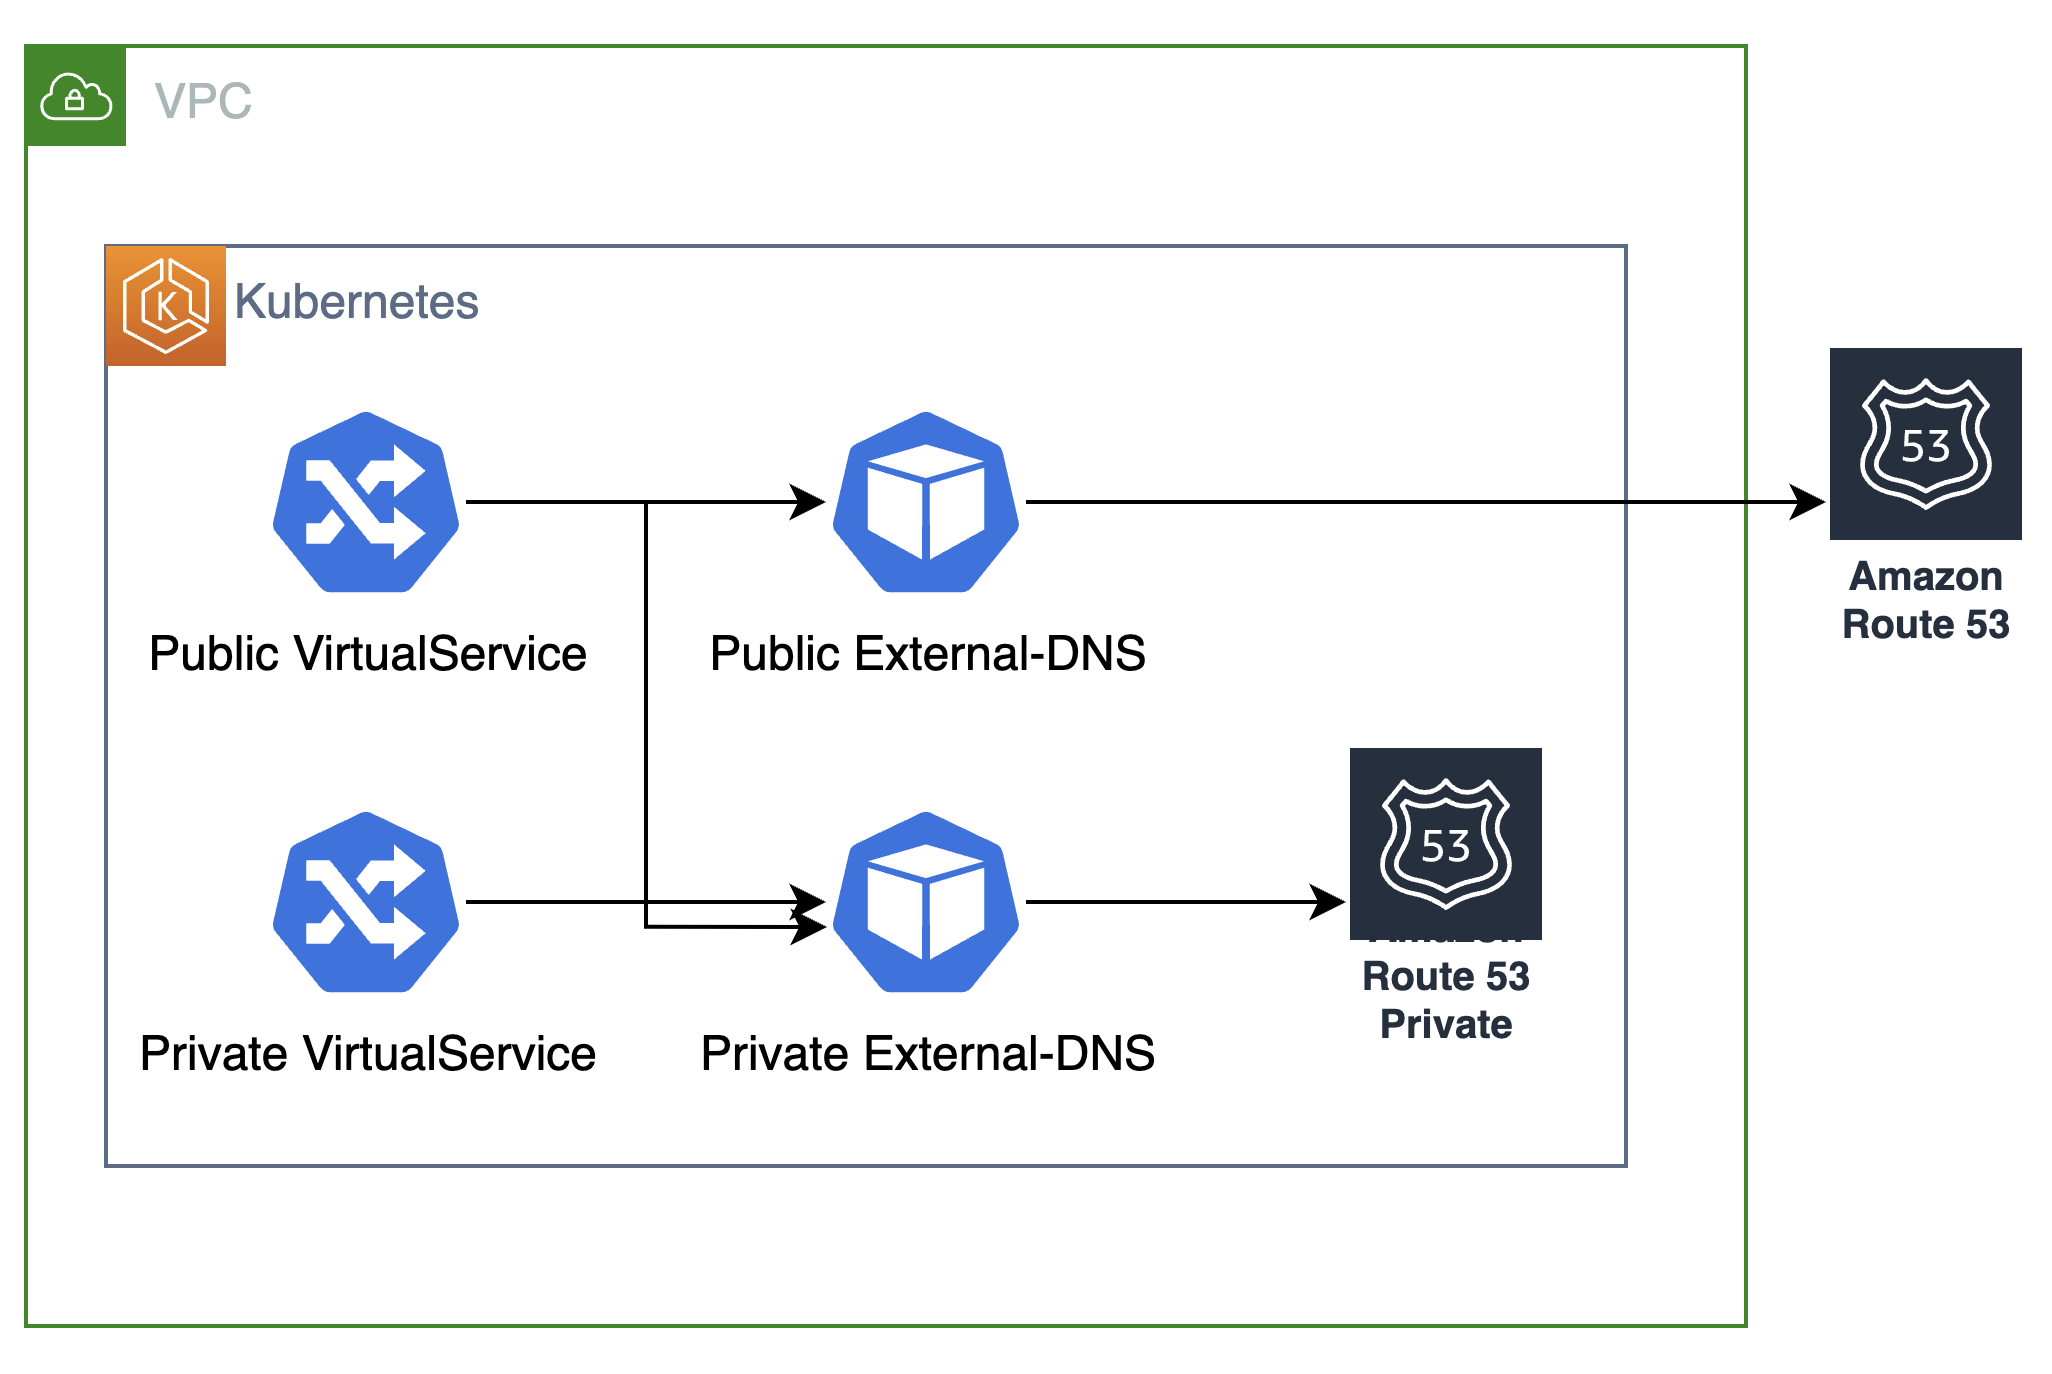
\includegraphics[width=0.9\textwidth]{gfx/now-external-dns}
    \caption{Private und öffentliche Zonenverwaltung mit external-dns}
    \label{fig:Projektbeschreibung:external-dns}
\end{figure}

Ein in Kubernetes veröffentlichter Service, zum Beispiel \enquote{service1}, wird in der VirtualService Resource mit der Subdomain \enquote{service1.dev.projekt1.sda-se.io} angegeben und als öffentlicher Service konfiguriert in dem es an das öffentliche Istio Ingress Gateway gebunden wird.
So wird der Service mit seiner Subdomain in sowohl der öffentlichen als auch der privaten Zone erstellt.
\medskip

Die Sicherheit der Zonen wird durch die Verwendung von \ac{DNSSEC} gewährleistet.
DNSSEC ist eine Erweiterung von DNS, welche die Authentizität und Integrität von DNS-Einträgen gewährleistet und somit die Sicherheit erhöht ~\cite{kelm2001sicherheit}.
Um bei AWS DNSSEC zu aktivieren, muss ein KMS-Schlüssel erstellt werden, welcher für die Signierung der DNS-Einträge verwendet wird.
Dieser Schlüssel wird in der Route53 Zone angegeben und aktiviert DNSSEC für diese Zone.
Außerdem muss eine Kette des Vertrauens erstellt werden, welche durch \enquote{DS} Records in der jeweiligen Übergeordneten Zone hinterlegt werden.
Nachfolgend wird die Verwaltung der öffentlichen Zonen beispielhaft mit Terraform dargestellt.
Es handelt sich um ein vereinfachtes Beispiel, welches die wesentlichen Teile der Konfiguration darstellt aber nicht so komplex ist, wie die tatsächliche Konfiguration.
\medskip

\lstinputlisting[language=Python,frame=tb,caption={DNSSEC mit Terraform},label={lst:dnssec-terraform}]{code/dnssec.tf}

\subsection{Analyse}
\label{subsec:description:analyse}
(Soll-/ Ist-Vergleich)

\subsection{Wirtschaftlichkeitsbetrachtung}
\label{subsec:description:ergebnisse:wirtschaftlichkeitsbetrachtung}
(Soll-/ Ist-Vergleich)

\section{Schlussfolgerung}
\label{sec:description:schlussfolgerung}
blablabla

\subsection{Auswirkungen}
\label{subsec:description:auswirkungen}
(Soll-/ Ist-Vergleich)

\subsection{Modifikationen}
\label{subsec:description:modifikationen}
(Soll-/ Ist-Vergleich)

\subsection{Bilanz}
\label{subsec:description:bilanz}
(Soll-/ Ist-Vergleich)

%*************************************************************************
% Recommendations
%*************************************************************************
%\part{Empfehlungen zur Erstellung wissenschaftlicher Abschlussarbeiten}
%\label{pt:recommendations}
%*************************************************************************
% Backmatter
%*************************************************************************
\appendix
%\renewcommand{\thechapter}{\alph{chapter}}
\cleardoublepage
\part{Appendix}
%************************************************
\chapter{Introduction to the ClassicThesis style}\label{ch:classicthesis}
%************************************************
The ClassicThesis bundle for \LaTeX\ has two goals:
\begin{enumerate}
    \item Provide students with an easy-to-use template for their
    Master's
    or PhD thesis. (Though it might also be used by other types of
    authors
    for reports, books, etc.)
    \item Provide a classic, high-quality typographic style that is
    inspired by \citeauthor{bringhurst:2002}'s ``\emph{The Elements of
    Typographic Style}'' \citep{bringhurst:2002}.
    \marginpar{\myTitle \myVersion}
\end{enumerate}
The bundle is configured to run with a \emph{full}
MiK\TeX\ or \TeX Live\footnote{See the file \texttt{LISTOFFILES} for
needed packages. Furthermore, \texttt{classicthesis}
works with most other distributions and, thus, with most systems
\LaTeX\ is available for.}
installation right away and, therefore, it uses only freely available
fonts. (Minion fans can easily adjust the style to their needs.)

People interested only in the nice style and not the whole bundle can
now use the style stand-alone via the file \texttt{classicthesis.sty}.
This works now also with \enquote{plain} \LaTeX.

As of version 3.0, \texttt{classicthesis} can also be easily used with
\mLyX\footnote{\url{http://www.lyx.org}} thanks to Nicholas Mariette
and Ivo Pletikosić. The \mLyX\ version of this manual will contain
more information on the details.

This should enable anyone with a basic knowledge of \LaTeXe\ or \mLyX\ to
produce beautiful documents without too much effort. In the end, this
is my overall goal: more beautiful documents, especially theses, as I
am tired of seeing so many ugly ones.

The whole template and the used style is released under the
\acsfont{GNU} General Public License.

If you like the style then I would appreciate a postcard:
\begin{center}
    André Miede \\
    Detmolder Straße 32 \\
    31737 Rinteln \\
    Germany
\end{center}
The postcards I received so far are available at:
\begin{center}
    \url{http://postcards.miede.de}
\end{center}
\marginpar{A well-balanced line width improves the legibility of
the text. That's what typography is all about, right?}
So far, many theses, some books, and several other publications have
been typeset successfully with it. If you are interested in some
typographic details behind it, enjoy Robert Bringhurst's wonderful book.
% \citep{bringhurst:2002}.

\paragraph{Important Note:} Some things of this style might look
unusual at first glance, many people feel so in the beginning.
However, all things are intentionally designed to be as they are,
especially these:
\begin{itemize}
    \item No bold fonts are used. Italics or spaced small caps do the
    job quite well.
    \item The size of the text body is intentionally shaped like it
    is. It supports both legibility and allows a reasonable amount of
    information to be on a page. And, no: the lines are not too short.
    \item The tables intentionally do not use vertical or double
    rules. See the documentation for the \texttt{booktabs} package for
    a nice discussion of this topic.\footnote{To be found online at
    \url{http://mirror.ctan.org/macros/latex/contrib/booktabs/}.}
    \item And last but not least, to provide the reader with a way
    easier access to page numbers in the table of contents, the page
    numbers are right behind the titles. Yes, they are \emph{not}
    neatly aligned at the right side and they are \emph{not} connected
    with dots that help the eye to bridge a distance that is not
    necessary. If you are still not convinced: is your reader
    interested in the page number or does she want to sum the numbers
    up?
\end{itemize}
Therefore, please do not break the beauty of the style by changing
these things unless you really know what you are doing! Please.

\paragraph{Yet Another Important Note:} Since \texttt{classicthesis}'
first release in 2006, many things have changed in the \LaTeX\ world.
Trying to keep up-to-date, \texttt{classicthesis} grew and evolved
into many directions, trying to stay (some kind of) stable and be
compatible with its port to \mLyX. However, there are still many
remains from older times in the code, many dirty workarounds here and
there, and several other things I am absolutely not proud of (for
example my unwise combination of \acsfont{KOMA} and
\texttt{titlesec} etc.).
\graffito{An outlook into the future of \texttt{classicthesis}.}

Currently, I am looking into how to completely re-design and
re-implement \texttt{classicthesis} making it easier to maintain and
to use. As a general idea, \texttt{classicthesis.sty} should be
developed and distributed separately from the template bundle itself.
Excellent spin-offs such as \texttt{arsclassica} could also be
integrated (with permission by their authors) as format configurations.
Also, current trends of \texttt{microtype}, \texttt{fontspec}, etc.
should be included as well. As I am not really into deep
\LaTeX\ programming,
I will reach out to the \LaTeX\ community for their expertise and help.


\section{Organization}\label{sec:organization}
A very important factor for successful thesis writing is the
organization of the material. This template suggests a structure as
the following:
\begin{itemize}
    \marginpar{You can use these margins for summaries of the text
    body\dots}
    \item\texttt{Chapters/} is where all the \enquote{real} content goes in
    separate files such as \texttt{Chapter01.tex} etc.
    % \item\texttt{Examples/} is where you store all listings and other
    % examples you want to use for your text.
    \item\texttt{FrontBackMatter/} is where all the stuff goes that
    surrounds the \enquote{real} content, such as the acknowledgments,
    dedication, etc.
    \item\texttt{gfx/} is where you put all the graphics you use in
    the thesis. Maybe they should be organized into subfolders
    depending on the chapter they are used in, if you have a lot of
    graphics.
    \item\texttt{Bibliography.bib}: the Bib\TeX\ database to organize
    all the references you might want to cite.
    \item\texttt{classicthesis.sty}: the style definition to get this
    awesome look and feel. Does not only work with this thesis template
    but also on its own (see folder \texttt{Examples}). Bonus: works
    with both \LaTeX\ and \textsc{pdf}\LaTeX\dots and \mLyX.
    % \item\texttt{ClassicThesis.tcp} a \TeX nicCenter project file.
    Great tool and it's free!
    \item\texttt{ClassicThesis.tex}: the main file of your thesis
    where all gets bundled together.
    \item\texttt{classicthesis-config.tex}: a central place to load all
    nifty packages that are used. % In there, you can also activate
    % backrefs in order to have information in the bibliography about
    % where a source was cited in the text (\ie, the page number).

    \emph{Make your changes and adjustments here.} This means that you
    specify here the options you want to load \texttt{classicthesis.sty}
    with. You also adjust the title of your thesis, your name, and all
    similar information here. Refer to \cref{sec:customization} for more
    information.

    This had to change as of version 3.0 in order to enable an easy
    transition from the \enquote{basic} style to \mLyX.
\end{itemize}
In total, this should get you started in no time.


\clearpage
\section{Style Options}\label{sec:style-options}
There are a couple of options for \texttt{classicthesis.sty} that
allow for a bit of freedom concerning the layout:
\marginpar{\dots or your supervisor might use the margins for some
    comments of her own while reading.}
\begin{itemize}
    \item General:
        \begin{itemize}
            \item\texttt{drafting}: prints the date and time at the bottom of
            each page, so you always know which version you are dealing with.
            Might come in handy not to give your Prof. that old draft.
        \end{itemize}

    \item Parts and Chapters:
        \begin{itemize}
            \item\texttt{parts}: if you use Part divisions for your document,
            you should choose this option. (Cannot be used together with
            \texttt{nochapters}.)

            \item\texttt{linedheaders}: changes the look of the chapter
            headings a bit by adding a horizontal line above the chapter
            title. The chapter number will also be moved to the top of the
            page, above the chapter title.
        \end{itemize}

    \item Typography:
        \begin{itemize}
            \item\texttt{eulerchapternumbers}: use figures from Hermann Zapf's
            Euler math font for the chapter numbers. By default, old style
            figures from the Palatino font are used.

            \item\texttt{beramono}: loads Bera Mono as typewriter font.
            (Default setting is using the standard CM typewriter font.)

            \item\texttt{eulermath}: loads the awesome Euler fonts for math.
            Pala\-tino is used as default font.
        \end{itemize}

    \marginpar{Options are enabled via \texttt{option=true}}

    \item Table of Contents:
        \begin{itemize}
            \item\texttt{tocaligned}: aligns the whole table of contents on
            the left side. Some people like that, some don't.

            \item\texttt{dottedtoc}: sets pagenumbers flushed right in the
            table of contents.

            \item\texttt{manychapters}: if you need more than nine chapters for
            your document, you might not be happy with the spacing between the
            chapter number and the chapter title in the Table of Contents.
            This option allows for additional space in this context.
            However, it does not look as \enquote{perfect} if you use
            \verb|\parts| for structuring your document.
        \end{itemize}

    \item Floats:
        \begin{itemize}
            \item\texttt{listings}: loads the \texttt{listings} package (if not
            already done) and configures the List of Listings accordingly.

            \item\texttt{floatperchapter}: activates numbering per chapter for
            all floats such as figures, tables, and listings (if used).
        \end{itemize}

\end{itemize}

Furthermore, pre-defined margins for different paper sizes are available, \eg, \texttt{a4paper}, \texttt{a5paper}, and \texttt{letterpaper}. These are based on your chosen option of \verb|\documentclass|.

The best way to figure these options out is to try the different
possibilities and see what you and your supervisor like best.

In order to make things easier, \texttt{classicthesis-config.tex}
contains some useful commands that might help you.


\section{Customization}\label{sec:customization}
%(As of v3.0, the Classic Thesis Style for \LaTeX{} and \mLyX{} share
%the same two \texttt{.sty} files.)
This section will show you some hints how to adapt
\texttt{classicthesis} to your needs.

The file \texttt{classicthesis.sty}
contains the core functionality of the style and in most cases will
be left intact, whereas the file \texttt{classic\-thesis-config.tex}
is used for some common user customizations.

The first customization you are about to make is to alter the document
title, author name, and other thesis details. In order to do this, replace
the data in the following lines of \texttt{classicthesis-config.tex:}%
\marginpar{Modifications in \texttt{classic\-thesis-config.tex}%
}

\begin{lstlisting}
    % **************************************************
    % 2. Personal data and user ad-hoc commands
    % **************************************************
    \newcommand{\myTitle}{A Classic Thesis Style\xspace}
    \newcommand{\mySubtitle}{An Homage to...\xspace}
\end{lstlisting}

Further customization can be made in \texttt{classicthesis-config.tex}
by choosing the options to \texttt{classicthesis.sty}
in a line that looks like this:

\begin{lstlisting}[label={lst:lstlisting}]
  \PassOptionsToPackage{
    drafting=true,    % print version information on the bottom of the pages
    tocaligned=false, % the left column of the toc will be aligned (no indentation)
    dottedtoc=false,  % page numbers in ToC flushed right
    parts=true,       % use part division
    eulerchapternumbers=true, % use AMS Euler for chapter font (otherwise Palatino)
    linedheaders=false,       % chaper headers will have line above and beneath
    floatperchapter=true,     % numbering per chapter for all floats (i.e., Figure 1.1)
    listings=true,    % load listings package and setup LoL
    subfig=true,      % setup for preloaded subfig package
    eulermath=false,  % use awesome Euler fonts for mathematical formulae (only with pdfLaTeX)
    beramono=true,    % toggle a nice monospaced font (w/ bold)
    minionpro=false   % setup for minion pro font; use minion pro small caps as well (only with pdfLaTeX)
  }{classicthesis}
\end{lstlisting}

Many other customizations in \texttt{classicthesis-config.tex} are
possible, but you should be careful making changes there, since some
changes could cause errors.

% Finally, changes can be made in the file \texttt{classicthesis.sty},%
% \marginpar{Modifications in \texttt{classicthesis.sty}%
% } although this is mostly not designed for user customization. The
% main change that might be made here is the text-block size, for example,
% to get longer lines of text.


\section{Issues}\label{sec:issues}
This section will list some information about problems using
\texttt{classic\-thesis} in general or using it with other packages.

Beta versions of \texttt{classicthesis} can be found at Bitbucket:
\begin{center}
    \url{https://bitbucket.org/amiede/classicthesis/}
\end{center}
There, you can also post serious bugs and problems you encounter.


\section{Future Work}\label{sec:future-work}
So far, this is a quite stable version that served a couple of people
well during their thesis time. However, some things are still not as
they should be. Proper documentation in the standard format is still
missing. In the long run, the style should probably be published
separately, with the template bundle being only an application of the
style. Alas, there is no time for that at the moment\dots it could be
a nice task for a small group of \LaTeX nicians.

Please do not send me email with questions concerning \LaTeX\ or the
template, as I do not have time for an answer. But if you have
comments, suggestions, or improvements for the style or the template
in general, do not hesitate to write them on that postcard of yours.


\section{Beyond a Thesis}\label{sec:beyond-a-thesis}
The layout of \texttt{classicthesis.sty} can be easily used without the
framework of this template. A few examples where it was used to typeset
an article, a book or a curriculum vitae can be found in the folder
\texttt{Examples}. The examples have been tested with
\texttt{latex} and \texttt{pdflatex} and are easy to compile. To
encourage you even more, PDFs built from the sources can be found in the
same folder.


\section{License}\label{sec:license}

\paragraph{GNU General Public License:} This program is free software;
you can redistribute it and/or modify
it under the terms of the \acsfont{GNU} General Public License as
published by
the Free Software Foundation; either version 2 of the License, or
(at your option) any later version.

This program is distributed in the hope that it will be useful,
but \emph{without any warranty}; without even the implied warranty of
\emph{merchant\-ability} or \emph{fitness for a particular purpose}.
See the
\acsfont{GNU} General Public License for more details.

You should have received a copy of the \acsfont{GNU} General
Public License
along with this program; see the file \texttt{COPYING}.  If not,
write to
the Free Software Foundation, Inc., 59 Temple Place - Suite 330,
Boston, MA 02111-1307, USA.

\paragraph{classichthesis Authors' note:} There have been some discussions about the GPL's implications on using \texttt{classicthesis} for theses etc. Details can be found here:
\begin{center}
  \url{https://bitbucket.org/amiede/classicthesis/issues/123/}
\end{center}

We chose (and currently stick with) the GPL because we would not like to compete with proprietary modified versions of our own work. However, the whole template is free as free beer and free speech. We will not demand the sources for theses, books, CVs, etc. that were created using \texttt{classicthesis}.

Postcards are still highly appreciated.





%*****************************************
%*****************************************
%*****************************************
%*****************************************
%*****************************************

%********************************************************************
% Appendix
%*******************************************************
% If problems with the headers: get headings in appendix etc. right
%\markboth{\spacedlowsmallcaps{Appendix}}{\spacedlowsmallcaps{Appendix}}
\chapter{Appendix Test}
Lorem ipsum at nusquam appellantur his, ut eos erant homero
concludaturque. Albucius appellantur deterruisset id eam, vivendum
partiendo dissentiet ei ius. Vis melius facilisis ea, sea id convenire
referrentur, takimata adolescens ex duo. Ei harum argumentum per. Eam
vidit exerci appetere ad, ut vel zzril intellegam interpretaris.
\graffito{More dummy text.}

%Errem omnium ea per, pro congue populo ornatus cu, ex qui dicant
%nemore melius. No pri diam iriure euismod. Graecis eleifend
%appellantur quo id. Id corpora inimicus nam, facer nonummy ne pro,
%kasd repudiandae ei mei. Mea menandri mediocrem dissentiet cu, ex
%nominati imperdiet nec, sea odio duis vocent ei. Tempor everti
%appareat cu ius, ridens audiam an qui, aliquid admodum conceptam ne
%qui. Vis ea melius nostrum, mel alienum euripidis eu.

\section{Appendix Section Test}\label{sec:appendix-section-test}
Test: \cref{tab:moreexample} (This reference should have a
lowercase, small caps \spacedlowsmallcaps{A} if the option
\texttt{floatperchapter} is activated, just as in the table itself
 $\rightarrow$ however, this does not work at the moment.)

\begin{table}[h]
    \myfloatalign
    \begin{tabularx}{\textwidth}{Xll} \toprule
        \tableheadline{labitur bonorum pri no} & \tableheadline{que vista}
        & \tableheadline{human} \\ \midrule
        fastidii ea ius & germano &  demonstratea \\
        suscipit instructior & titulo & personas \\
        %postulant quo & westeuropee & sanctificatec \\
        \midrule
        quaestio philosophia & facto & demonstrated \\
        %autem vulputate ex & parola & romanic \\
        %usu mucius iisque & studio & sanctificatef \\
        \bottomrule
    \end{tabularx}
    \caption[Autem usu id]{Autem usu id.}
    \label{tab:moreexample}
\end{table}

%Nulla fastidii ea ius, exerci suscipit instructior te nam, in ullum
%postulant quo. Congue quaestio philosophia his at, sea odio autem
%vulputate ex. Cu usu mucius iisque voluptua. Sit maiorum propriae at,
%ea cum primis intellegat. Hinc cotidieque reprehendunt eu nec. Autem
%timeam deleniti usu id, in nec nibh altera.




\section{Another Appendix Section Test}\label{sec:another-appendix-section-test}
Equidem detraxit cu nam, vix eu delenit periculis. Eos ut vero
constituto, no vidit propriae complectitur sea. Diceret nonummy in
has, no qui eligendi recteque consetetur. Mel eu dictas suscipiantur,
et sed placerat oporteat. At ipsum electram mei, ad aeque atomorum
mea. There is also a useless Pascal listing below: \cref{lst:useless}.

\begin{lstlisting}[float=b,language=Pascal,frame=tb,caption={A floating example (\texttt{listings} manual)},label=lst:useless]
for i:=maxint downto 0 do
begin
{ do nothing }
end;
\end{lstlisting}

%Ei solet nemore consectetuer nam. Ad eam porro impetus, te choro omnes
%evertitur mel. Molestie conclusionemque vel at, no qui omittam
%expetenda efficiendi. Eu quo nobis offendit, verterem scriptorem ne
%vix.

%*************************************************************************
% Other Stuff in the Back
%*************************************************************************
\cleardoublepage\include{frontbackmatter/Bibliography}
%*************************************************************************
% Game Over: Restore, Restart, or Quit?
%*************************************************************************
\end{document}
%*************************************************************************
